\documentclass[11pt,letterpaper]{article}
\usepackage[margin=0.87in]{geometry}
\usepackage[T1]{fontenc}
\usepackage{lmodern}
\usepackage{microtype}
\usepackage{amsmath}
\usepackage{xcolor}
\usepackage{graphicx}
\usepackage{tikz}
\usepackage{pgfplots}
\pgfplotsset{compat=1.18}
\usetikzlibrary{arrows.meta,calc,positioning,patterns,decorations.pathmorphing,shapes.misc}
\usepackage{booktabs,tabularx,array}
\usepackage{float}
\usepackage{needspace}
\usepackage[font=small,labelfont=bf,labelsep=period,skip=4pt]{caption}
\usepackage{fancyhdr}
\usepackage[colorlinks=true,linkcolor=teal!65!black,urlcolor=teal!65!black,citecolor=teal!65!black]{hyperref}

% Palette
\definecolor{ink}{HTML}{17324D}
\definecolor{accent}{HTML}{176B70}
\definecolor{pale}{HTML}{EDF5F4}
\definecolor{curl}{HTML}{C8742B}     % the curled arrangement
\definecolor{curlpale}{HTML}{F6E3D3}
\definecolor{flat}{HTML}{2E7D8C}     % the flat arrangement
\definecolor{flatpale}{HTML}{D6ECF0}
\definecolor{melt}{HTML}{8E6C8A}     % the random phase
\definecolor{meltpale}{HTML}{E9DEE8}
\definecolor{sun}{HTML}{E0A526}
\definecolor{no}{HTML}{B03A2E}
\definecolor{kExact}{HTML}{176B70}
\definecolor{kMeas}{HTML}{2F5F9E}
\definecolor{kPub}{HTML}{5A5A5A}
\definecolor{kOurs}{HTML}{9A5B00}
\definecolor{kClaim}{HTML}{8A2D5A}

\setlength{\parindent}{0pt}
\setlength{\parskip}{0.62em}
\renewcommand{\baselinestretch}{1.08}
\setlength{\headheight}{14pt}
\pagestyle{fancy}
\fancyhf{}
\fancyhead[L]{\small\color{ink}The curled torus burps}
\fancyhead[R]{\small Plain-language edition}
\fancyfoot[C]{\small\thepage}
\renewcommand{\headrulewidth}{0.3pt}
\hypersetup{pdftitle={The curled torus burps: the story behind the experiment},pdfauthor={Emily Smith}}

% Chapter opener, sub-heading, take-away box
\newcommand{\chapterpage}[2]{\par\Needspace{16\baselineskip}\vspace{1.4em}{\color{accent}\small\textbf{#1}}\par\vspace{0.2em}{\color{ink}\LARGE\bfseries #2}\par\vspace{0.5em}}
\newcommand{\takeaway}[1]{\par\medskip\noindent\colorbox{pale}{\parbox{\dimexpr\linewidth-2\fboxsep\relax}{\vspace{0.35em}\textbf{The point to keep:} #1\vspace{0.35em}}}\par\medskip}
\newcommand{\whyhere}[1]{\par\medskip\noindent{\color{accent}\small\textbf{Why we went here.}} {\small #1}\par\medskip}
\newcommand{\sub}[1]{\par\medskip{\color{ink}\large\bfseries #1}\par}

% Kinds of statement (project rule 10), as small tags
\newcommand{\tagbox}[2]{{\sffamily\scriptsize\colorbox{#1}{\textcolor{white}{\strut #2}}}}
\newcommand{\Exact}{\tagbox{kExact}{EXACT}}
\newcommand{\Meas}{\tagbox{kMeas}{MEASURED}}
\newcommand{\MeasX}{\tagbox{kMeas}{MEASURED, EXPLORATORY}}
\newcommand{\Pub}{\tagbox{kPub}{PUBLISHED}}
\newcommand{\Ours}{\tagbox{kOurs}{OUR READING, UNVERIFIED}}
\newcommand{\Claim}{\tagbox{kClaim}{THE AUTHOR'S CLAIM}}
\newcommand{\Sketch}{\tagbox{kPub}{SKETCH, NOT DATA}}

\begin{document}
\thispagestyle{empty}
{\color{accent}\small\textbf{THE STORY BEHIND THE EXPERIMENT}}\par
\vspace{1em}
{\color{ink}\fontsize{29}{33}\selectfont\bfseries The curled torus burps}\par
\vspace{0.5em}
{\raggedright\Large A small push, a large release,\\and the question of what survives\par}
\vspace{0.7em}
\textbf{Emily Smith}\quad Independent researcher\par
10 October 2026 \enspace\textbullet\enspace Plain-language edition of the technical paper of the same date~\cite{tech}
\vspace{0.9em}

Everything you have ever seen happened in flat space: three directions you can move in. We know its
rules well. What we do not know is how it came to be.

This paper is about a hypothetical change: space emerging sharply from something else. We want to
understand that change, and how the two phases of being are related. We engage a toy model of dots
and links and ask three questions: what does it take to start such a change, what comes out when it
happens, and what is left behind.

\begin{figure}[H]
\centering
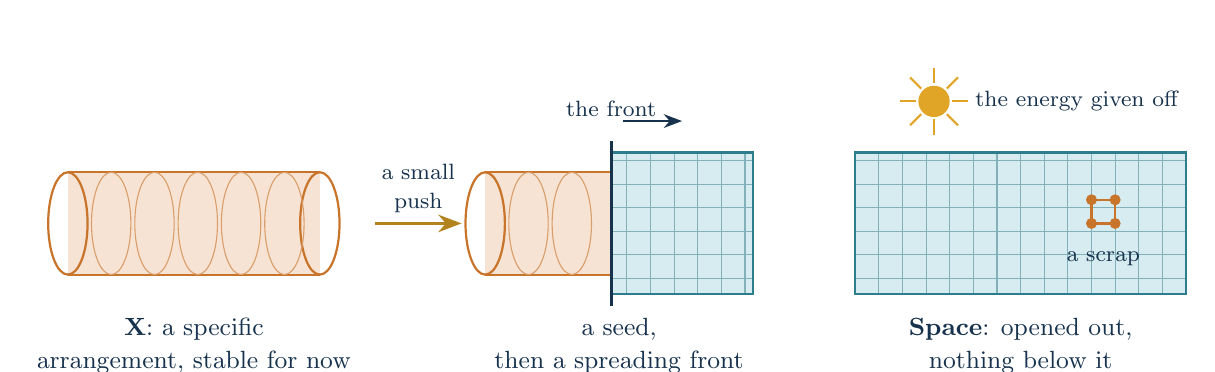
\begin{tikzpicture}[x=1cm,y=1cm,>=Stealth,font=\small]
% --- X: the tube
\begin{scope}[shift={(0,0)}]
\fill[curlpale] (0,0.35) rectangle (3.2,1.65);
\draw[curl,thick] (0,0.35) -- (3.2,0.35) (0,1.65) -- (3.2,1.65);
\draw[curl,thick] (0,1) ellipse (0.25 and 0.65);
\draw[curl,thick] (3.2,1) ellipse (0.25 and 0.65);
\foreach \x in {0.55,1.1,...,2.8} {\draw[curl!70] (\x,1) ellipse (0.25 and 0.65);}
\node[text=ink,align=center] at (1.6,-0.55) {\textbf{X}: a specific\\arrangement, stable for now};
\end{scope}
% --- push
\draw[->,very thick,sun!80!black] (3.9,1) -- (5.0,1) node[midway,above,text=ink,align=center,font=\footnotesize] {a small\\push};
% --- the change: front
\begin{scope}[shift={(5.3,0)}]
\fill[curlpale] (0,0.35) rectangle (1.6,1.65);
\draw[curl,thick] (0,0.35) -- (1.6,0.35) (0,1.65) -- (1.6,1.65);
\draw[curl,thick] (0,1) ellipse (0.25 and 0.65);
\foreach \x in {0.55,1.1} {\draw[curl!70] (\x,1) ellipse (0.25 and 0.65);}
\fill[flatpale] (1.6,0.1) -- (3.4,0.1) -- (3.4,1.9) -- (1.6,1.9) -- cycle;
\draw[flat!60,step=0.3] (1.6,0.1) grid (3.4,1.9);
\draw[flat,thick] (1.6,0.1) rectangle (3.4,1.9);
\draw[very thick,ink] (1.6,-0.05) -- (1.6,2.05);
\node[text=ink,font=\footnotesize,align=center] at (1.6,2.45) {the front};
\draw[->,thick,ink] (1.75,2.3) -- (2.5,2.3);
\node[text=ink,align=center] at (1.7,-0.55) {a seed,\\then a spreading front};
\end{scope}
% --- space
\begin{scope}[shift={(10.0,0)}]
\fill[flatpale] (0,0.1) rectangle (4.2,1.9);
\draw[flat!60,step=0.3] (0,0.1) grid (4.2,1.9);
\draw[flat,thick] (0,0.1) rectangle (4.2,1.9);
% sun: the burp
\node[circle,fill=sun,inner sep=4pt] (sun) at (1.0,2.55) {};
\foreach \a in {0,45,...,315} {\draw[sun,thick] (sun) ++(\a:0.23) -- ++(\a:0.2);}
\node[text=ink,font=\footnotesize,anchor=west] at (1.4,2.55) {the energy given off};
% scrap
\foreach \p in {(3.0,1.0),(3.3,1.0),(3.0,1.3),(3.3,1.3)} {\fill[curl] \p circle (0.07);}
\draw[curl,thick] (3.0,1.0) -- (3.3,1.0) -- (3.3,1.3) -- (3.0,1.3) -- cycle;
\node[text=ink,font=\footnotesize,align=center] at (3.15,0.55) {a scrap};
\node[text=ink,align=center] at (2.1,-0.55) {\textbf{Space}: opened out,\\nothing below it};
\end{scope}
\end{tikzpicture}
\caption{The idea in one picture. \Sketch\ What came before space, called X here (left), waits until a
small push starts it; the new arrangement spreads behind a front (middle); when it is done, flat space holds the energy
that came out plus a small scrap of the old arrangement (right). Everything in this paper is a test of
some part of this picture inside one toy model. The total energy is the same before and after.
Chapter~3 says why X is drawn as a tube.}
\label{fig:idea}
\end{figure}

\sub{Who is saying what}
The project keeps four kinds of statement apart, and this edition tags them where it matters, so
that a sentence is never quietly promoted from one kind to another. One more tag marks other
people's published work.
\begin{itemize}\setlength{\itemsep}{1pt}
\item \Exact\ Arithmetic, or a complete listing of every possibility. True of the model whatever a
run does.
\item \Meas\ A simulation whose rules and predictions were written down before it ran, with its
verdict. \MeasX\ means a run that was not formally pre-registered: its prediction was only written
into its configuration, or it is a closer look at runs already read.
\item \Pub\ Other researchers' published results.
\item \Ours\ A reading of a result, offered by the author and her AI assistants and checked by no
physicist. \Claim\ The author's hypothesis about reality, stated as hers.
\end{itemize}
Numbers in square brackets point to the sources listed at the end.

\chapterpage{1 \enspace THE PLACE WE START}{We live in flat space, and we cannot rerun its birth}

\Pub\ Measured at the largest scales, our universe is flat: the angles of enormous triangles add up to
what school geometry says they should, to within the precision of the best sky surveys~\cite{Planck18}.
It has three large directions. Its rules are known: general relativity for gravity and the shape of
space, quantum mechanics for everything small.

What is not known is how such a thing comes to exist. Candidate theories say that space is not the
stage on which everything happens but a \emph{phase} of something deeper, the way ice is a phase of
water. If that is right, there was a change, and changes come in two kinds.

\Pub\ Cool water, and nothing much happens until it reaches zero degrees. Then it freezes, giving off
heat as it goes, with ice and water side by side for a while. Very clean water can even stay liquid
below zero, stuck behind a hill it cannot climb on its own, until a jolt sets it off. Heat a fridge
magnet instead and its pull fades away: no hill, no burst of heat, no moment when half of it has
changed. Physicists call the first kind \textbf{first order} and the second \textbf{continuous}.
Plainer words: sharp and smooth.

\begin{figure}[H]
\centering
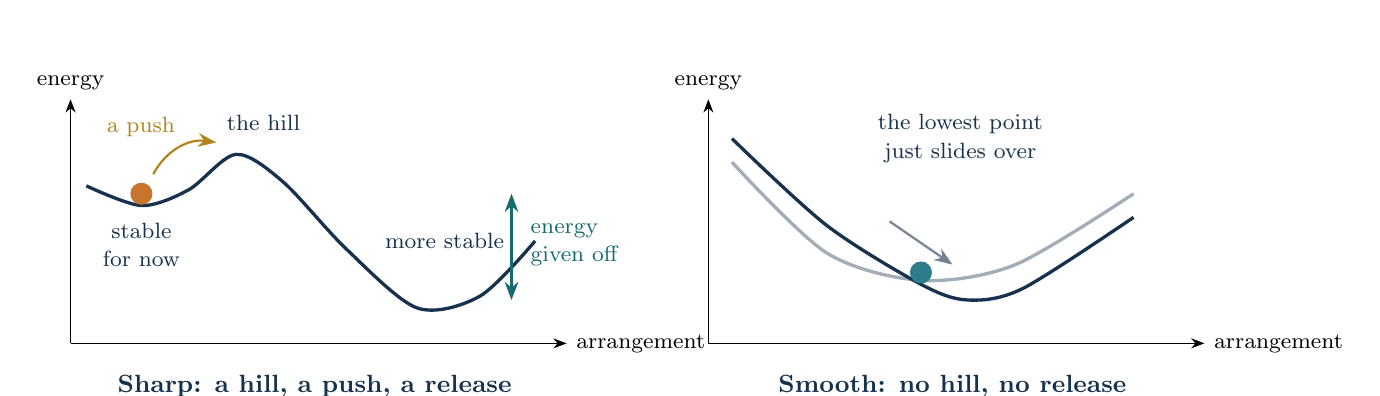
\begin{tikzpicture}[x=1cm,y=1cm,>=Stealth,font=\small]
% left: sharp
\begin{scope}
\draw[->] (0,0) -- (0,3.1) node[above,font=\footnotesize] {energy};
\draw[->] (0,0) -- (6.3,0) node[right,font=\footnotesize] {arrangement};
\draw[very thick,ink] plot[smooth] coordinates {(0.2,2.0) (0.9,1.75) (1.5,1.95) (2.1,2.4) (2.7,2.05) (3.5,1.2) (4.4,0.45) (5.2,0.6) (5.9,1.3)};
\fill[curl] (0.9,1.9) circle (0.14);
\node[font=\footnotesize,align=center,text=ink] at (0.9,1.25) {stable\\for now};
\node[font=\footnotesize,align=center,text=ink] at (2.45,2.8) {the hill};
\draw[->,thick,sun!80!black] (1.05,2.15) to[bend left=35] (1.85,2.55);
\node[font=\footnotesize,text=sun!80!black,anchor=south east] at (1.45,2.5) {a push};
\draw[<->,thick,accent] (5.6,0.55) -- (5.6,1.9);
\node[font=\footnotesize,align=left,text=accent,anchor=west] at (5.72,1.25) {energy\\given off};
\node[font=\footnotesize,align=center,text=ink] at (4.75,1.3) {more stable};
\node[font=\small\bfseries,text=ink] at (3.1,-0.55) {Sharp: a hill, a push, a release};
\end{scope}
% right: smooth
\begin{scope}[shift={(8.1,0)}]
\draw[->] (0,0) -- (0,3.1) node[above,font=\footnotesize] {energy};
\draw[->] (0,0) -- (6.3,0) node[right,font=\footnotesize] {arrangement};
\draw[very thick,ink!40] plot[smooth] coordinates {(0.3,2.3) (1.5,1.15) (2.7,0.8) (3.9,1.0) (5.4,1.9)};
\draw[very thick,ink] plot[smooth] coordinates {(0.3,2.6) (1.5,1.5) (2.7,0.75) (3.3,0.55) (4.0,0.7) (5.4,1.6)};
\fill[flat] (2.7,0.9) circle (0.14);
\draw[->,thick,ink!60] (2.3,1.55) -- (3.1,1.0);
\node[font=\footnotesize,align=center,text=ink] at (3.2,2.6) {the lowest point\\just slides over};
\node[font=\small\bfseries,text=ink] at (3.1,-0.55) {Smooth: no hill, no release};
\end{scope}
\end{tikzpicture}
\caption{The two kinds of change, as a ball on a landscape. \Sketch\ Height is energy; the ball is the
system. Left: a sharp change waits in a hollow, needs a push to clear the rim, and then falls a
definite distance, which is the energy it gives off. Right: a smooth change has no rim and no drop;
the best arrangement drifts. This paper is about the left-hand kind.}
\label{fig:landscape}
\end{figure}

How do you tell which kind you have? \Pub\ Let the system jiggle for a long time and count how often
it turns up at each energy. A sharp change shows two humps with a valley between, because the system
is almost always in one state or the other. A smooth change shows one hump.

\begin{figure}[H]
\centering
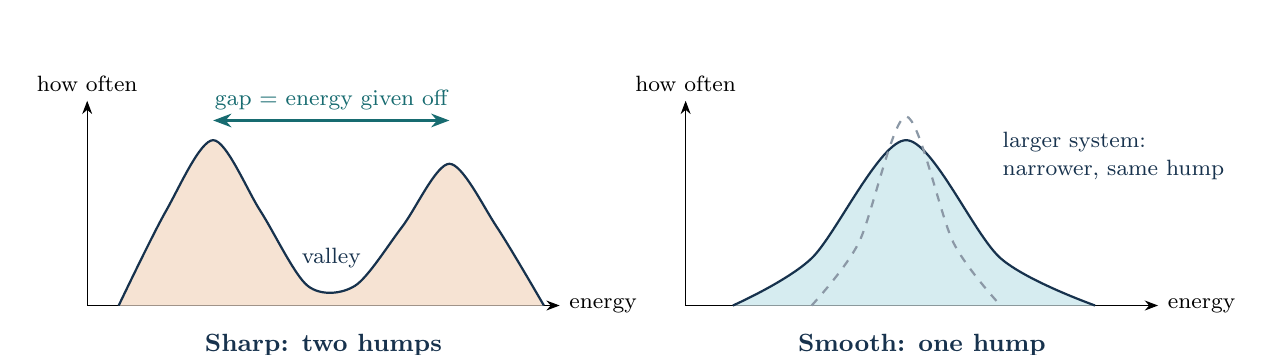
\begin{tikzpicture}[x=1cm,y=1cm,>=Stealth,font=\small]
\begin{scope}
\draw[->] (0,0) -- (0,2.6) node[above,font=\footnotesize] {how often};
\draw[->] (0,0) -- (6,0) node[right,font=\footnotesize] {energy};
\fill[curlpale] plot[smooth] coordinates {(0.4,0) (1.0,1.2) (1.6,2.1) (2.2,1.2) (2.8,0.25) (3.4,0.25) (4.0,1.0) (4.6,1.8) (5.2,1.0) (5.8,0)} -- cycle;
\draw[thick,ink] plot[smooth] coordinates {(0.4,0) (1.0,1.2) (1.6,2.1) (2.2,1.2) (2.8,0.25) (3.4,0.25) (4.0,1.0) (4.6,1.8) (5.2,1.0) (5.8,0)};
\draw[<->,thick,accent] (1.6,2.35) -- (4.6,2.35) node[midway,above,font=\footnotesize,text=accent] {gap = energy given off};
\node[font=\footnotesize,text=ink] at (3.1,0.6) {valley};
\node[font=\small\bfseries,text=ink] at (3,-0.5) {Sharp: two humps};
\end{scope}
\begin{scope}[shift={(7.6,0)}]
\draw[->] (0,0) -- (0,2.6) node[above,font=\footnotesize] {how often};
\draw[->] (0,0) -- (6,0) node[right,font=\footnotesize] {energy};
\fill[flatpale] plot[smooth] coordinates {(0.6,0) (1.6,0.6) (2.8,2.1) (4.0,0.6) (5.2,0)} -- cycle;
\draw[thick,ink] plot[smooth] coordinates {(0.6,0) (1.6,0.6) (2.8,2.1) (4.0,0.6) (5.2,0)};
\draw[thick,ink!50,dashed] plot[smooth] coordinates {(1.6,0) (2.2,0.8) (2.8,2.4) (3.4,0.8) (4.0,0)};
\node[font=\footnotesize,text=ink,align=left,anchor=west] at (3.9,1.9) {larger system:\\narrower, same hump};
\node[font=\small\bfseries,text=ink] at (3,-0.5) {Smooth: one hump};
\end{scope}
\end{tikzpicture}
\caption{What a long run measures. \Sketch\ The valley of the left-hand picture is the hill of
Figure~\ref{fig:landscape} seen from underneath: states that cost extra are states the system rarely
visits. The distance between the humps is the energy a sharp change gives off.}
\label{fig:humps}
\end{figure}

Two things make this hard. Small systems hide the hill: with only a few pieces, everything can flip at
once, so even a sharp change looks like one broad hump. And the real test is whether the valley
deepens as the system grows, which needs sizes nobody can simulate cheaply. Still, we set out a series
of simulations that let us describe a sharp change of this kind in some detail.

Here is the author's idea, in one paragraph. First, who is asking, and why. She is a software
engineer, not a physicist, and also a startup founder and a foster mom, so her recreational time is
scarce and the computing bills are her own. The project is called RecreationalPhysics anyway. Her
reason is simple: she wants to map her intuition about how reality is organized onto what humanity
knows about the universe.

\Claim\ Space is one settled arrangement of something deeper, which she calls X because nobody knows
what it is. X was not chaos. It was a specific arrangement, stable for now, the way a reagent is
stable until something gives it a push. The change that made space was sharp: it started at a seed,
spread as a front, released a definite amount of energy that became matter and light, and left a
remainder. Across the change the energy books balance.

That paragraph is a hypothesis, not a result, and nothing in a computer can prove it about reality.
What a computer can do is take a model in which space is an arrangement of links, and ask whether a
change of this kind can happen in it at all: whether there is a hill, how high it is, what comes
down the far side, and what the far side is like. If the answer were no, the idea would have no home
in that model. If the answer is yes, the idea gains a laboratory, and every number in it becomes a
thing to check.

\takeaway{We cannot rerun the birth of space, so we build a toy in which space is an arrangement and
ask what \emph{kind} of change produces it. The author's idea needs the sharp kind: a hill, a push, a
release of energy, a remainder.}

\chapterpage{2 \enspace THE TOY}{A published model of space made of links}

\Pub\ The model is called combinatorial quantum gravity, built by Carlo Trugenberger, Christy Kelly
and Fabio Biancalana~\cite{T17,KTB19,T25}. It is a network of dots and links with no positions at all: a
dot has no place, only neighbors. Figure~\ref{fig:model} shows every rule it has. The mathematical
word for such a thing is a \textbf{graph}; its dots are vertices, its links are edges.

\begin{figure}[H]
\centering
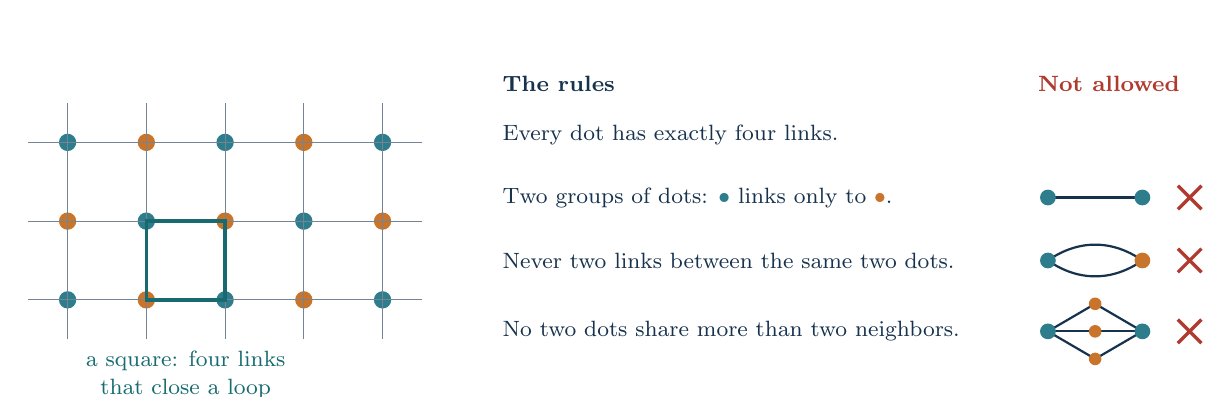
\begin{tikzpicture}[x=1cm,y=1cm,font=\small]
\foreach \i in {0,...,4} \foreach \j in {0,...,2} {
  \pgfmathparse{int(mod(\i+\j,2))}
  \ifnum\pgfmathresult=0 \fill[flat] (\i,\j) circle (0.11); \else \fill[curl] (\i,\j) circle (0.11); \fi }
\foreach \i in {0,...,3} \foreach \j in {0,...,2} {\draw[ink!60] (\i,\j) -- (\i+1,\j);}
\foreach \i in {0,...,4} \foreach \j in {0,...,1} {\draw[ink!60] (\i,\j) -- (\i,\j+1);}
\draw[ink!60] (0,0) -- (-0.5,0) (0,1) -- (-0.5,1) (0,2) -- (-0.5,2) (4,0) -- (4.5,0) (4,1) -- (4.5,1) (4,2) -- (4.5,2);
\foreach \i in {0,...,4} {\draw[ink!60] (\i,2) -- (\i,2.5) (\i,0) -- (\i,-0.5);}
\draw[very thick,accent] (1,0) -- (2,0) -- (2,1) -- (1,1) -- cycle;
\node[font=\footnotesize,text=accent,align=center] at (1.5,-0.95) {a square: four links\\that close a loop};
% the rules, each with what it forbids
\node[font=\footnotesize\bfseries,text=ink,anchor=west] at (5.4,2.75) {The rules};
\node[font=\footnotesize\bfseries,text=no,anchor=west] at (12.2,2.75) {Not allowed};
\node[font=\footnotesize,text=ink,align=left,anchor=west] at (5.4,2.1) {Every dot has exactly four links.};
\node[font=\footnotesize,text=ink,align=left,anchor=west] at (5.4,1.3) {Two groups of dots: \textcolor{flat}{$\bullet$} links only to \textcolor{curl}{$\bullet$}.};
\node[font=\footnotesize,text=ink,align=left,anchor=west] at (5.4,0.5) {Never two links between the same two dots.};
\node[font=\footnotesize,text=ink,align=left,anchor=west] at (5.4,-0.4) {No two dots share more than two neighbors.};
\begin{scope}[shift={(0.45,0)}]
% not allowed: a link inside one group
\draw[thick,ink] (12.0,1.3) -- (13.2,1.3);
\fill[flat] (12.0,1.3) circle (0.1); \fill[flat] (13.2,1.3) circle (0.1);
\draw[no,very thick] (13.65,1.15) -- (13.95,1.45) (13.65,1.45) -- (13.95,1.15);
% not allowed: two links between the same two dots
\draw[thick,ink] (12.0,0.5) to[bend left=35] (13.2,0.5);
\draw[thick,ink] (12.0,0.5) to[bend right=35] (13.2,0.5);
\fill[flat] (12.0,0.5) circle (0.1); \fill[curl] (13.2,0.5) circle (0.1);
\draw[no,very thick] (13.65,0.35) -- (13.95,0.65) (13.65,0.65) -- (13.95,0.35);
% not allowed: two dots sharing three neighbors
\foreach \y in {-0.05,-0.4,-0.75} {\draw[thick,ink] (12.0,-0.4) -- (12.6,\y) -- (13.2,-0.4); \fill[curl] (12.6,\y) circle (0.08);}
\fill[flat] (12.0,-0.4) circle (0.1); \fill[flat] (13.2,-0.4) circle (0.1);
\draw[no,very thick] (13.65,-0.55) -- (13.95,-0.25) (13.65,-0.25) -- (13.95,-0.55);
\end{scope}
\end{tikzpicture}
\caption{The whole model: dots, four links each, two groups, and the loops of four links called
squares. There are no positions. Drawing the dots on a grid is a convenience; only the links are
real.}
\label{fig:model}
\end{figure}

\sub{The price list}
\Pub\ The model gives every arrangement an energy, and the energy is worked out by counting squares.
Compared with an arrangement that has one square for every dot, every missing square has a cost. A
single link may carry at most three squares; a link carrying a third one has one square too many, and
every such surplus square has a cost of its own. Those two prices are the entire rule. To be clear,
this energy has no meters or joules in it. We will just call its amount a \textbf{unit}, and leave the
conversion of units into physical energy for a later paper. Everything below is in these units.

\Pub\ A missing square costs 16 units. A surplus square costs $4\lambda$ units, where $\lambda$
(lambda) is a number that sets the surplus price. It can be turned up or down, so we call it
\textbf{the knob}. At exactly $\lambda = 1$ a surplus square costs 4, and the energy is then a measure
of how curved the network is: a graph version of the curvature in Einstein's equations of gravity.
That is where the model's name comes from, a theory of gravity built by combinatorics, the mathematics
of counting. The published work also studies a simpler version with the surplus price switched off,
$\lambda = 0$, where a link can carry a third square for free. Turning the knob to other values is our
addition.

The whole point of the published program is to get general relativity, Einstein's theory of gravity,
back out of a network, so the curvature setting is the one that matters to it. At any other
$\lambda$, however, the energy is still a perfectly good rule for a network, but it is no longer a
curvature. So everything in this paper at $\lambda \neq 1$ is a close cousin of combinatorial quantum
gravity, not the thing itself.

We have not found published work that sets the surplus price to any value above 1~\cite{search}. In
print, as far as we have found, are the two settings just described and, in the text of two of the
papers~\cite{KTB19,KT19}, a version in which a third square is forbidden outright. So, barring a gap in
our search, the approach taken here and what it turned up are new.

\begin{figure}[H]
\centering
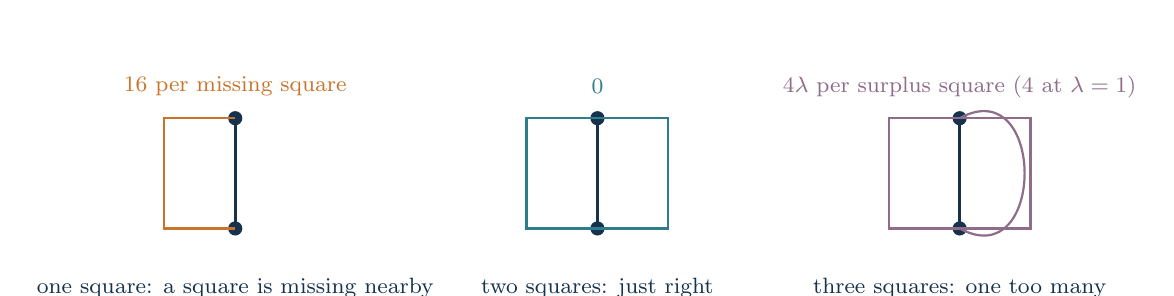
\begin{tikzpicture}[x=1cm,y=1cm,font=\small]
\foreach \k/\lab/\price/\col in {0/one square: a square is missing nearby/costs/curl,4.6/two squares: just right/costs nothing/flat,9.2/three squares: one too many/costs/melt} {
 \begin{scope}[shift={(\k,0)}]
  \draw[very thick,ink] (1.5,0.2) -- (1.5,1.6);
  \fill[ink] (1.5,0.2) circle (0.09) (1.5,1.6) circle (0.09);
  \draw[\col,thick] (1.5,0.2) -- (0.6,0.2) -- (0.6,1.6) -- (1.5,1.6);
  \node[font=\footnotesize,text=ink,align=center] at (1.5,-0.55) {\lab};
 \end{scope}}
\begin{scope}[shift={(4.6,0)}] \draw[flat,thick] (1.5,0.2) -- (2.4,0.2) -- (2.4,1.6) -- (1.5,1.6); \end{scope}
\begin{scope}[shift={(9.2,0)}] \draw[melt,thick] (1.5,0.2) -- (2.4,0.2) -- (2.4,1.6) -- (1.5,1.6);
  \draw[melt,thick] (1.5,0.2) .. controls (2.6,-0.4) and (2.6,2.2) .. (1.5,1.6); \end{scope}
\node[font=\footnotesize,text=curl] at (1.5,2.0) {16 per missing square};
\node[font=\footnotesize,text=flat] at (6.1,2.0) {0};
\node[font=\footnotesize,text=melt] at (10.7,2.0) {$4\lambda$ per surplus square (4 at $\lambda=1$)};
\end{tikzpicture}
\caption{The price list, read link by link. \Exact\ The thick link carries one, two or three squares.
Two is free. Fewer means a square is missing nearby, at 16 per missing square; a third is a surplus
square, at $4\lambda$, set by the knob. At $\lambda = 1$ the two prices make the energy a measure of
the network's curvature; at $\lambda = 0$ a third square is free.}
\label{fig:prices}
\end{figure}

\sub{The one move}
The network cannot leap to a new arrangement. \Pub\ It changes by \textbf{swapping partners}: pick
two links, Alice--Ben and Cara--Dan, and rewire them as Alice--Dan and Cara--Ben. Every dot keeps its
four links and its group. Any swap that breaks the other rules is thrown out. That is the only move.

\begin{figure}[H]
\centering
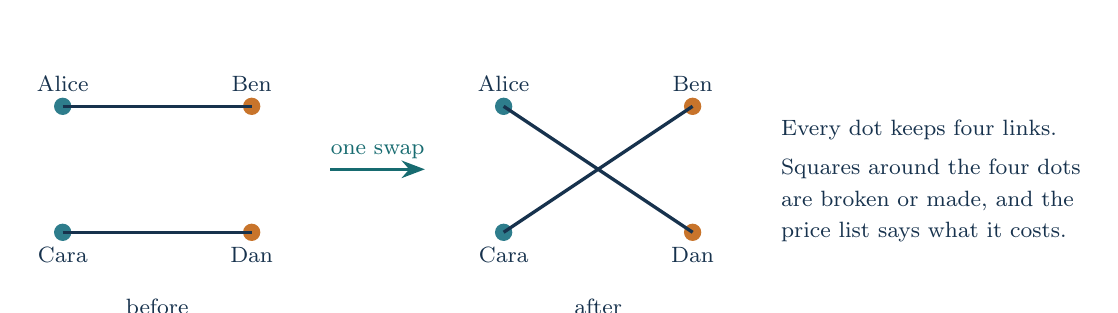
\begin{tikzpicture}[x=1cm,y=1cm,font=\small,>=Stealth]
\begin{scope}
\fill[flat] (0,1.6) circle (0.11) node[above=2pt,text=ink,font=\footnotesize] {Alice};
\fill[flat] (0,0) circle (0.11) node[below=2pt,text=ink,font=\footnotesize] {Cara};
\fill[curl] (2.4,1.6) circle (0.11) node[above=2pt,text=ink,font=\footnotesize] {Ben};
\fill[curl] (2.4,0) circle (0.11) node[below=2pt,text=ink,font=\footnotesize] {Dan};
\draw[very thick,ink] (0,1.6) -- (2.4,1.6) (0,0) -- (2.4,0);
\node[font=\footnotesize,text=ink] at (1.2,-0.95) {before};
\end{scope}
\draw[->,very thick,accent] (3.4,0.8) -- (4.6,0.8) node[midway,above,font=\footnotesize,text=accent] {one swap};
\begin{scope}[shift={(5.6,0)}]
\fill[flat] (0,1.6) circle (0.11) node[above=2pt,text=ink,font=\footnotesize] {Alice};
\fill[flat] (0,0) circle (0.11) node[below=2pt,text=ink,font=\footnotesize] {Cara};
\fill[curl] (2.4,1.6) circle (0.11) node[above=2pt,text=ink,font=\footnotesize] {Ben};
\fill[curl] (2.4,0) circle (0.11) node[below=2pt,text=ink,font=\footnotesize] {Dan};
\draw[very thick,ink] (0,1.6) -- (2.4,0) (0,0) -- (2.4,1.6);
\node[font=\footnotesize,text=ink] at (1.2,-0.95) {after};
\end{scope}
\node[font=\footnotesize,text=ink,align=left,anchor=west] at (9.0,1.3) {Every dot keeps four links.};
\node[font=\footnotesize,text=ink,align=left,anchor=west] at (9.0,0.8) {Squares around the four dots};
\node[font=\footnotesize,text=ink,align=left,anchor=west] at (9.0,0.4) {are broken or made, and the};
\node[font=\footnotesize,text=ink,align=left,anchor=west] at (9.0,0.0) {price list says what it costs.};
\end{tikzpicture}
\caption{The one move the network has. \Pub\ Two links swap partners. Everything that happens in the
rest of this paper is a long chain of these.}
\label{fig:swap}
\end{figure}

\sub{Warmth, and the bath}
\Pub\ A run of the model is a long chain of such swaps, each one proposed at random and then accepted
or refused. A second number, $g$, decides which. It plays the part of temperature, and we call it
\textbf{the warmth}. A swap that lowers the energy is always accepted. A swap that raises it by
$\Delta E$ units is accepted only some of the time, with a chance of $e^{-\Delta E/g}$, where $e$ is a
fixed number, about 2.7: the bigger the cost, the rarer the swap, and the warmer the network, the more
often it goes through. Picture the network sitting in a bath that lends it energy for an uphill swap
and takes back whatever a downhill swap gives off. The bath is endless: it never runs out and never
fills up. Lowering $g$ is cooling the network. Time in a run is counted in \textbf{sweeps}: one sweep
is two proposed swaps for every dot. Rules of this kind are the standard way to sample such a model;
they are not a claim about how anything moved in real time.

\sub{The question the field asks, and reproduction as a starting point}
\Pub\ Start from a random tangle of links, cool it slowly, and watch. Does geometry condense out of the
tangle sharply, with two humps, or smoothly? The published answers: with the full rule
($\lambda = 1$), smoothly~\cite{KTB19,T25}; with the surplus price switched off ($\lambda = 0$),
sharply, but the network breaks into many small closed pieces rather than one space~\cite{T25,GV21}.
With a third square free, cooling packs in as many squares as the rules allow, and the most tightly
packed arrangements close up on themselves; Chapter~3 shows what those pieces are. Kelly's doctoral
thesis~\cite{Kelly22} adds a hint for four links per dot: cooled and then warmed again, the network
does not quite retrace its path, a small but persistent gap of the kind a sharp change leaves, though
the thesis declines to call the evidence definitive.

\Meas\ We repeated this before anything else.\footnote{One published 2025 figure from the same
group~\cite{T25} disagrees with ours over one stretch, but it also disagrees with that group's own
2019 curve~\cite{KTB19}, so it is a question for them and is recorded as open.} Our simulations land
on the model's published 2019 curve~\cite{KTB19} to about half a percent at the same size, match exact
averages at sizes small enough to list every possible arrangement, and reproduce the sharp change into
closed pieces with the surplus price off. Then we measured how much energy the change gives off as the
tangle orders, at several sizes, with the rules written down first.

\begin{center}
\renewcommand{\arraystretch}{1.15}
\begin{tabular}{llr}
\toprule
Setting & Dots & Energy given off per dot as the tangle orders \\
\midrule
Surplus price off ($\lambda = 0$) & 48 & 10.3 \\
 & 64 & 11.3 \\
 & 96 & 12.5 \\
Full rule ($\lambda = 1$) & 36 & at most 1.65 \\
 & 64 & at most 1.51 \\
 & 100 & at most 1.30, and falling \\
\bottomrule
\end{tabular}
\end{center}

\Meas\ With the surplus price off, the energy given off is large and grows with size, but the cold
state is a pile of closed pieces, not a space. With the full rule, which does make a space, there is
one hump at every size we ran, and any energy given off is small and shrinking. Settings of 1.25 and
1.5 gave the same picture. We got the same answer the published work did, and added the comparison
across sizes that the 2019 paper said was out of reach.

\takeaway{The model's energy is a price list: 16 per missing square, $4\lambda$ per surplus square.
At $\lambda=1$ it is a curvature, which is why that setting is studied. Out of randomness, at that
setting, the change is smooth: no sign of a release of energy at the sizes anyone can reach.}

\chapterpage{3 \enspace THE PHASE BEFORE}{What if what came before space was not random?}

The published question starts from a random tangle. This program asks a different one: what if what
came before space was not random at all, but a specific arrangement, stable for now, with energy to
give? That question is the focus of everything that follows. To ask it in the toy, we first need to
say what space looks like in a network with no positions, and what the alternative to it could be.

\sub{Directions}
Space, at its simplest, is a set of large directions: directions you can keep walking in.
Figure~\ref{fig:pairs} shows how to find them in a network that has no positions.

\begin{figure}[H]
\centering
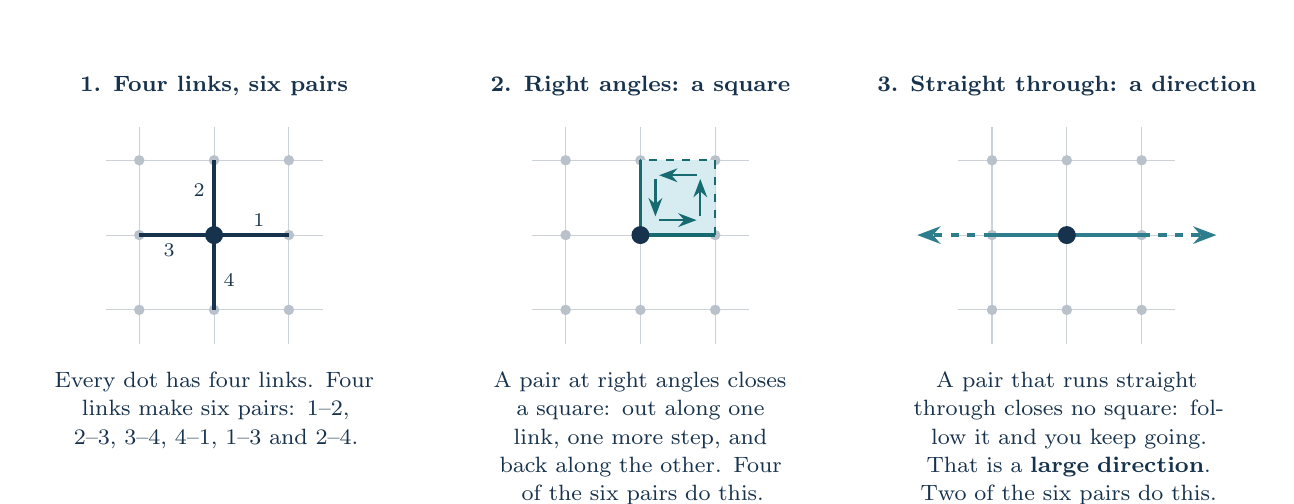
\begin{tikzpicture}[x=0.95cm,y=0.95cm,font=\footnotesize,>=Stealth]
\foreach \k/\ttl in {0/{1. Four links, six pairs},5.7/{2. Right angles: a square},11.4/{3. Straight through: a direction}} {
 \begin{scope}[shift={(\k,0)}]
  \foreach \i in {0,1,2} {\draw[ink!22] (\i,-0.45) -- (\i,2.45); \draw[ink!22] (-0.45,\i) -- (2.45,\i);}
  \foreach \i in {0,1,2} \foreach \j in {0,1,2} {\fill[ink!30] (\i,\j) circle (0.07);}
  \node[font=\footnotesize\bfseries,text=ink] at (1,3.0) {\ttl};
 \end{scope}}
% 1: the four links of one dot
\begin{scope}
 \foreach \a/\n in {0/1,90/2,180/3,270/4} {\draw[very thick,ink] (1,1) -- ++(\a:1); \node[text=ink,font=\scriptsize] at ($(1,1)+(\a:0.6)+(\a+90:0.2)$) {\n};}
 \fill[ink] (1,1) circle (0.12);
 \node[text=ink,align=center,text width=4.5cm,anchor=north] at (1,-0.7) {Every dot has four links. Four links make six pairs: 1--2, 2--3, 3--4, 4--1, 1--3 and 2--4.};
\end{scope}
% 2: a pair at right angles closes a square
\begin{scope}[shift={(5.7,0)}]
 \fill[flatpale] (1,1) rectangle (2,2);
 \draw[very thick,accent] (2,1) -- (1,1) -- (1,2);
 \draw[thick,accent,dashed] (2,1) -- (2,2) -- (1,2);
 \draw[->,accent,thick] (1.25,1.2) -- (1.75,1.2);
 \draw[->,accent,thick] (1.8,1.25) -- (1.8,1.75);
 \draw[->,accent,thick] (1.75,1.8) -- (1.25,1.8);
 \draw[->,accent,thick] (1.2,1.75) -- (1.2,1.25);
 \fill[ink] (1,1) circle (0.12);
 \node[text=ink,align=center,text width=4.5cm,anchor=north] at (1,-0.7) {A pair at right angles closes a square: out along one link, one more step, and back along the other. Four of the six pairs do this.};
\end{scope}
% 3: a pair straight through closes no square
\begin{scope}[shift={(11.4,0)}]
 \draw[very thick,flat] (0,1) -- (2,1);
 \draw[very thick,flat,dashed,->] (2,1) -- (3.0,1);
 \draw[very thick,flat,dashed,->] (0,1) -- (-1.0,1);
 \fill[ink] (1,1) circle (0.12);
 \node[text=ink,align=center,text width=4.5cm,anchor=north] at (1,-0.7) {A pair that runs straight through closes no square: follow it and you keep going. That is a \textbf{large direction}. Two of the six pairs do this.};
\end{scope}
\end{tikzpicture}
\caption{What a direction is, in a network with no positions. \Exact\ Count the pairs at a dot that
close no square, and call the count $d$. On a flat grid, $d = 2$.}
\label{fig:pairs}
\end{figure}

\sub{A grid with no edges}
A grid drawn on paper has edges, where the dots run out of links. The toy removes the edges.

\begin{figure}[H]
\centering
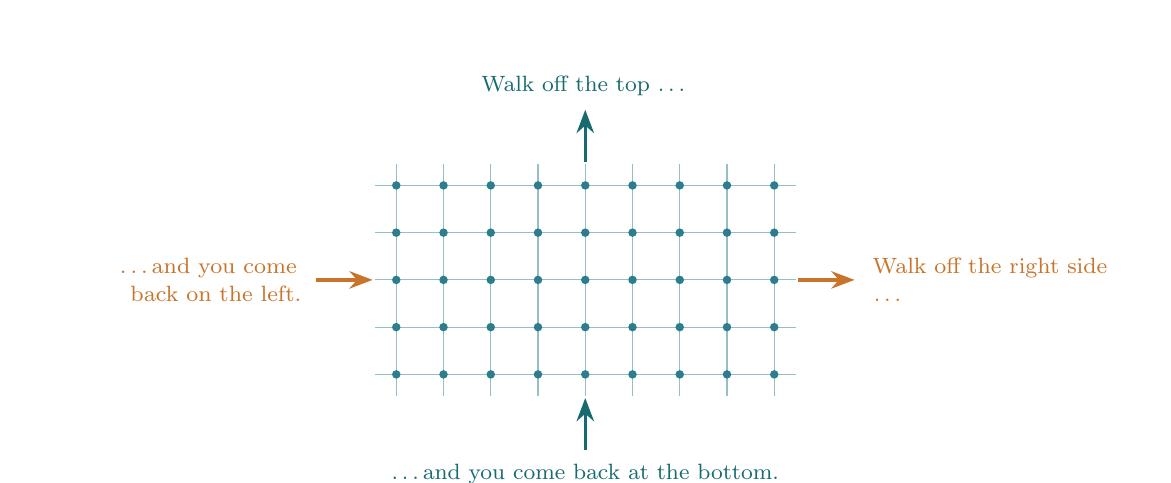
\begin{tikzpicture}[x=0.6cm,y=0.6cm,font=\footnotesize,>=Stealth]
\foreach \i in {0,...,8} {\draw[flat!50] (\i,-0.45) -- (\i,4.45);}
\foreach \j in {0,...,4} {\draw[flat!50] (-0.45,\j) -- (8.45,\j);}
\foreach \i in {0,...,8} \foreach \j in {0,...,4} {\fill[flat] (\i,\j) circle (0.09);}
% leaving on the right, entering on the left
\draw[->,very thick,curl] (8.5,2) -- (9.7,2);
\draw[->,very thick,curl] (-1.7,2) -- (-0.5,2);
\node[text=curl,anchor=west,align=left,text width=3.3cm] at (9.9,2) {Walk off the right side \ldots};
\node[text=curl,anchor=east,align=right,text width=3.3cm] at (-1.9,2) {\ldots and you come back on the left.};
% leaving at the top, entering at the bottom
\draw[->,very thick,accent] (4,4.5) -- (4,5.6);
\draw[->,very thick,accent] (4,-1.6) -- (4,-0.5);
\node[text=accent,anchor=south] at (4,5.7) {Walk off the top \ldots};
\node[text=accent,anchor=north] at (4,-1.7) {\ldots and you come back at the bottom.};
\end{tikzpicture}
\caption{The toy's flat space. \Exact\ The grid wraps around both ways, like an old game screen whose
edges join. It has no edges, so every dot has its four links, and when both ways around are long every
dot reads $d=2$. We call it \textbf{the flat sheet}. Mathematicians call any grid that wraps both ways a
\textbf{torus}. Every shape in this paper is a torus; this one is the flat kind.}
\label{fig:wrap}
\end{figure}

\sub{Curling}
If a direction is not large, what else can it be? Small: curled up on itself.

\begin{figure}[H]
\centering
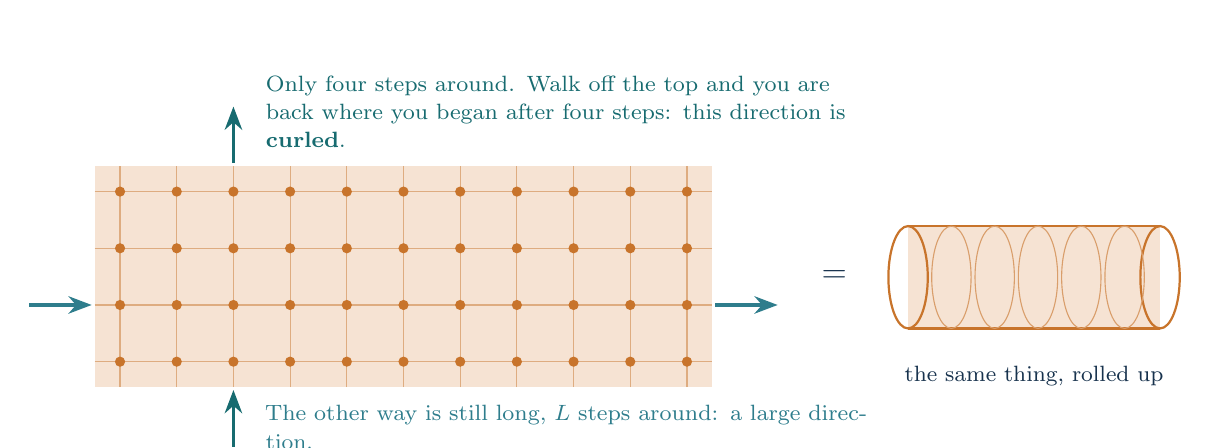
\begin{tikzpicture}[x=0.72cm,y=0.72cm,font=\footnotesize,>=Stealth]
% the tube drawn flat: 4 rows, 11 columns
\fill[curlpale] (-0.45,-0.45) rectangle (10.45,3.45);
\foreach \i in {0,...,10} {\draw[curl!60] (\i,-0.45) -- (\i,3.45);}
\foreach \j in {0,...,3} {\draw[curl!60] (-0.45,\j) -- (10.45,\j);}
\foreach \i in {0,...,10} \foreach \j in {0,...,3} {\fill[curl] (\i,\j) circle (0.09);}
% the short way around
\draw[->,very thick,accent] (2,3.5) -- (2,4.5);
\draw[->,very thick,accent] (2,-1.5) -- (2,-0.5);
\node[text=accent,anchor=south west,align=left,text width=7.6cm] at (2.4,3.6) {Only four steps around. Walk off the top and you are back where you began after four steps: this direction is \textbf{curled}.};
% the long way around
\draw[->,very thick,flat] (10.5,1) -- (11.6,1);
\draw[->,very thick,flat] (-1.6,1) -- (-0.5,1);
\node[text=flat,anchor=north west,align=left,text width=7.6cm] at (2.4,-0.6) {The other way is still long, $L$ steps around: a large direction.};
\node[text=ink,font=\large] at (12.6,1.5) {$=$};
% the same thing rolled up
\begin{scope}[shift={(13.9,0.1)},x=1cm,y=1cm]
 \fill[curlpale] (0,0.35) rectangle (3.2,1.65);
 \draw[curl,thick] (0,0.35) -- (3.2,0.35) (0,1.65) -- (3.2,1.65);
 \draw[curl,thick] (0,1) ellipse (0.25 and 0.65);
 \draw[curl,thick] (3.2,1) ellipse (0.25 and 0.65);
 \foreach \x in {0.55,1.1,...,2.8} {\draw[curl!70] (\x,1) ellipse (0.25 and 0.65);}
 \node[text=ink,align=center] at (1.6,-0.25) {the same thing, rolled up};
\end{scope}
\end{tikzpicture}
\caption{Curling one direction. \Exact\ Make one of the two ways around only four steps long. A grid
four dots around and $L$ dots along, wrapped both ways, is still a torus, the $4 \times L$ torus:
the curled kind. We call it \textbf{the tube}.}
\label{fig:tube}
\end{figure}

\begin{figure}[H]
\centering
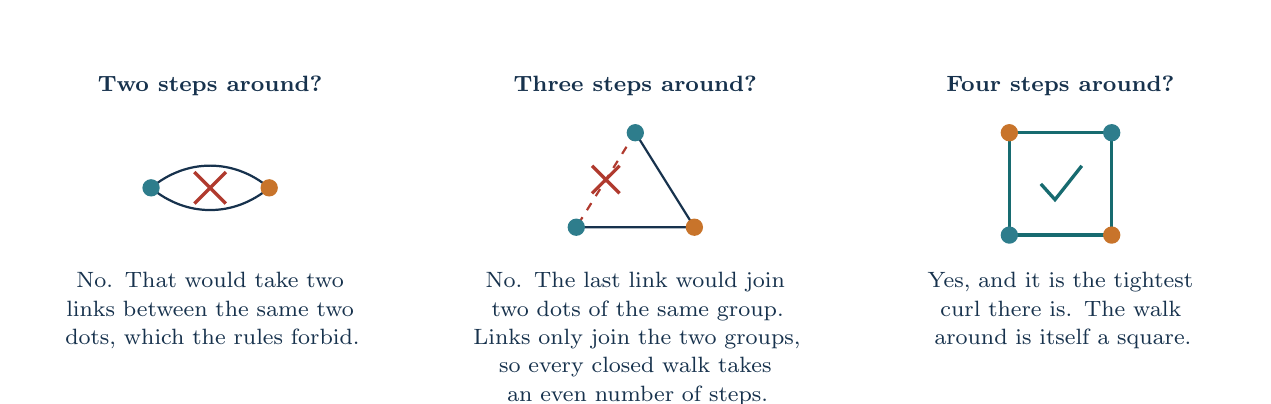
\begin{tikzpicture}[x=1cm,y=1cm,font=\footnotesize,>=Stealth]
% two steps around
\begin{scope}
 \draw[thick,ink] (0,0.7) to[bend left=40] (1.5,0.7);
 \draw[thick,ink] (0,0.7) to[bend right=40] (1.5,0.7);
 \fill[flat] (0,0.7) circle (0.11); \fill[curl] (1.5,0.7) circle (0.11);
 \draw[no,very thick] (0.55,0.5) -- (0.95,0.9) (0.55,0.9) -- (0.95,0.5);
 \node[font=\footnotesize\bfseries,text=ink] at (0.75,2.0) {Two steps around?};
 \node[text=ink,align=center,text width=4.4cm,anchor=north] at (0.75,-0.25) {No. That would take two links between the same two dots, which the rules forbid.};
\end{scope}
% three steps around
\begin{scope}[shift={(5.4,0)}]
 \draw[thick,ink] (0,0.2) -- (1.5,0.2) -- (0.75,1.4);
 \draw[thick,no,dashed] (0.75,1.4) -- (0,0.2);
 \fill[flat] (0,0.2) circle (0.11); \fill[curl] (1.5,0.2) circle (0.11); \fill[flat] (0.75,1.4) circle (0.11);
 \draw[no,very thick] (0.2,0.63) -- (0.55,0.98) (0.2,0.98) -- (0.55,0.63);
 \node[font=\footnotesize\bfseries,text=ink] at (0.75,2.0) {Three steps around?};
 \node[text=ink,align=center,text width=4.4cm,anchor=north] at (0.75,-0.25) {No. The last link would join two dots of the same group. Links only join the two groups, so every closed walk takes an even number of steps.};
\end{scope}
% four steps around
\begin{scope}[shift={(10.8,0)}]
 \draw[very thick,accent] (0.1,0.1) rectangle (1.4,1.4);
 \fill[flat] (0.1,0.1) circle (0.11); \fill[curl] (1.4,0.1) circle (0.11); \fill[flat] (1.4,1.4) circle (0.11); \fill[curl] (0.1,1.4) circle (0.11);
 \draw[accent,very thick] (0.5,0.75) -- (0.68,0.55) -- (1.02,0.98);
 \node[font=\footnotesize\bfseries,text=ink] at (0.75,2.0) {Four steps around?};
 \node[text=ink,align=center,text width=4.4cm,anchor=north] at (0.75,-0.25) {Yes, and it is the tightest curl there is. The walk around is itself a square.};
\end{scope}
\end{tikzpicture}
\caption{Why four steps around, and not three or two. \Exact}
\label{fig:whyfour}
\end{figure}

\begin{figure}[H]
\centering
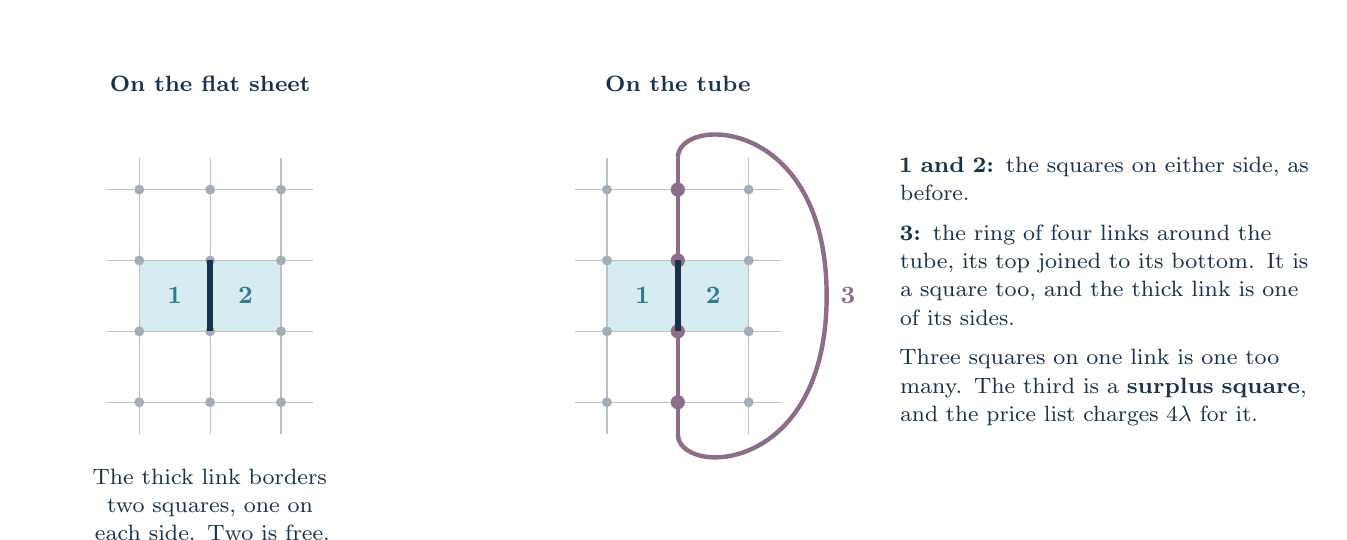
\begin{tikzpicture}[x=0.9cm,y=0.9cm,font=\footnotesize,>=Stealth]
% left: one link on the flat sheet
\begin{scope}
 \fill[flatpale] (0,1) rectangle (2,2);
 \foreach \i in {0,1,2} {\draw[ink!30] (\i,-0.45) -- (\i,3.45);}
 \foreach \j in {0,...,3} {\draw[ink!30] (-0.45,\j) -- (2.45,\j);}
 \foreach \i in {0,1,2} \foreach \j in {0,...,3} {\fill[ink!40] (\i,\j) circle (0.07);}
 \draw[line width=2pt,ink] (1,1) -- (1,2);
 \node[text=flat,font=\small\bfseries] at (0.5,1.5) {1};
 \node[text=flat,font=\small\bfseries] at (1.5,1.5) {2};
 \node[font=\footnotesize\bfseries,text=ink] at (1,4.5) {On the flat sheet};
 \node[text=ink,align=center,text width=4.4cm,anchor=north] at (1,-0.8) {The thick link borders two squares, one on each side. Two is free.};
\end{scope}
% right: the same link on the tube
\begin{scope}[shift={(6.6,0)}]
 \fill[flatpale] (0,1) rectangle (2,2);
 \foreach \i in {0,1,2} {\draw[ink!30] (\i,-0.45) -- (\i,3.45);}
 \foreach \j in {0,...,3} {\draw[ink!30] (-0.45,\j) -- (2.45,\j);}
 \foreach \i in {0,1,2} \foreach \j in {0,...,3} {\fill[ink!40] (\i,\j) circle (0.07);}
 % the ring: the four links of this column, its top joined to its bottom
 \draw[line width=1.6pt,melt] (1,-0.45) -- (1,3.45);
 \draw[line width=1.6pt,melt] (1,3.45) .. controls (1,4.05) and (3.1,4.05) .. (3.1,1.5) .. controls (3.1,-1.05) and (1,-1.05) .. (1,-0.45);
 \foreach \j in {0,...,3} {\fill[melt] (1,\j) circle (0.1);}
 \draw[line width=2.4pt,ink] (1,1) -- (1,2);
 \node[text=flat,font=\small\bfseries] at (0.5,1.5) {1};
 \node[text=flat,font=\small\bfseries] at (1.5,1.5) {2};
 \node[text=melt,font=\small\bfseries] at (3.4,1.5) {3};
 \node[font=\footnotesize\bfseries,text=ink] at (1,4.5) {On the tube};
 \node[text=ink,align=left,text width=5.2cm,anchor=north west] at (4.0,3.6) {\textbf{1 and 2:} the squares on either side, as before.\\[4pt]\textbf{3:} the ring of four links around the tube, its top joined to its bottom. It is a square too, and the thick link is one of its sides.\\[4pt]Three squares on one link is one too many. The third is a \textbf{surplus square}, and the price list charges $4\lambda$ for it.};
\end{scope}
\end{tikzpicture}
\caption{Curling puts a third square on a link. \Exact\ So curling a direction is exactly what the
surplus price charges for. And because the way around is now a square, the pair of links that points
that way closes one: the direction no longer counts as large, and every dot on the tube reads $d=1$.}
\label{fig:third}
\end{figure}

Curl both ways around to four steps and every dot reads $d = 0$: a closed sixteen-dot knot called the
4-cube. It is a torus too, curled both ways. Most of the closed pieces of Chapter~2 are these knots. Figure~\ref{fig:directions} puts the
three arrangements side by side.

\begin{figure}[H]
\centering
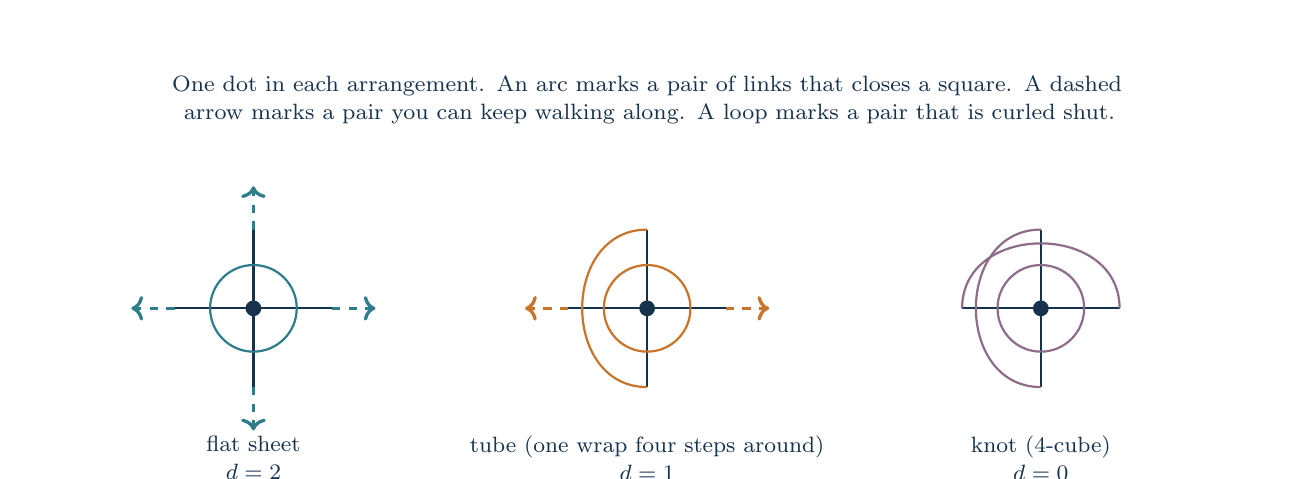
\begin{tikzpicture}[x=1cm,y=1cm,font=\small]
\foreach \k/\dd/\name/\col in {0/2/flat sheet/flat,5/1/tube (one wrap four steps around)/curl,10/0/knot (4-cube)/melt} {
 \begin{scope}[shift={(\k,0)}]
  \fill[ink] (1.5,1.2) circle (0.1);
  \foreach \a in {0,90,180,270} {\draw[thick,ink] (1.5,1.2) -- ++(\a:1.0);}
  % pairs at right angles always close squares: draw small arcs
  \foreach \a in {45,135,225,315} {\draw[\col,thick] (1.5,1.2) ++(\a-45:0.55) arc (\a-45:\a+45:0.55);}
  \node[font=\footnotesize,text=ink,align=center] at (1.5,-0.7) {\name\\$d = \dd$};
 \end{scope}}
% open directions: dashed arrows continuing beyond the link ends; curled: a loop joining the pair's ends
\begin{scope} \foreach \a in {0,90,180,270} {\draw[flat,dashed,very thick,->] (1.5,1.2) ++(\a:1.0) -- ++(\a:0.55);} \end{scope}
\begin{scope}[shift={(5,0)}] \foreach \a in {0,180} {\draw[curl,dashed,very thick,->] (1.5,1.2) ++(\a:1.0) -- ++(\a:0.55);} \draw[curl,thick] (1.5,0.2) .. controls (0.4,0.2) and (0.4,2.2) .. (1.5,2.2); \end{scope}
\begin{scope}[shift={(10,0)}] \draw[melt,thick] (1.5,0.2) .. controls (0.4,0.2) and (0.4,2.2) .. (1.5,2.2); \draw[melt,thick] (0.5,1.2) .. controls (0.5,2.3) and (2.5,2.3) .. (2.5,1.2); \end{scope}
\node[font=\footnotesize,text=ink,align=center,text width=15.5cm] at (6.5,3.85) {One dot in each arrangement. An arc marks a pair of links that closes a square. A dashed arrow marks a pair you can keep walking along. A loop marks a pair that is curled shut.};
\end{tikzpicture}

\vspace{0.5em}
{\footnotesize\color{ink}\textbf{This paper:} four links per dot, and the simplest change on the ladder: one curled direction opening ($d$ from 1 to 2).\par}
\vspace{0.7em}
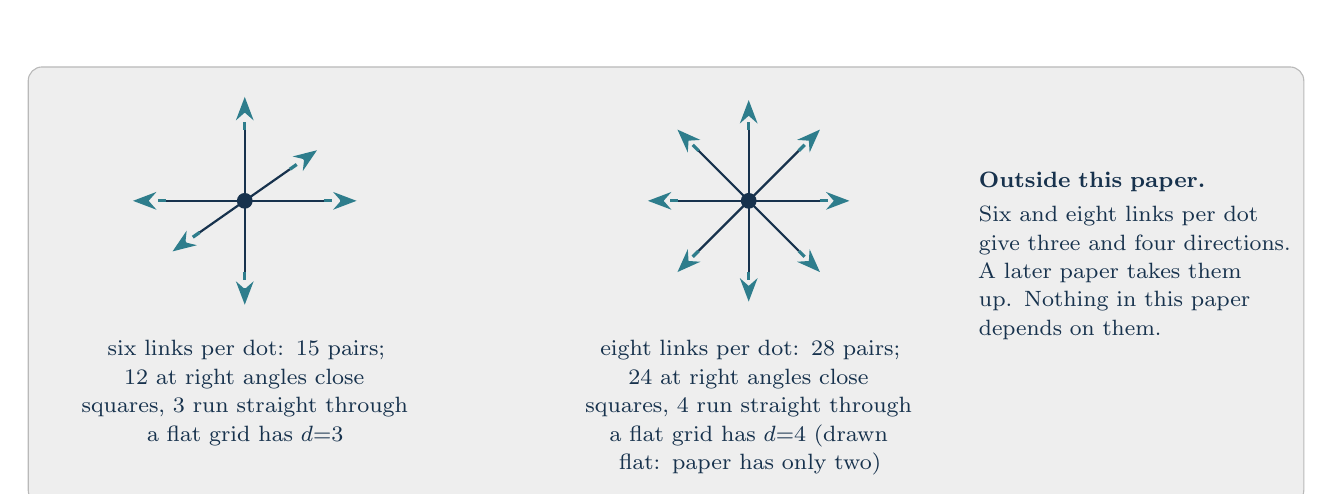
\begin{tikzpicture}[x=1cm,y=1cm,font=\small,>=Stealth]
% grey box: outside this paper's scope
\fill[gray!13,rounded corners=5pt] (-0.95,-2.55) rectangle (15.25,3.0);
\draw[gray!55,rounded corners=5pt] (-0.95,-2.55) rectangle (15.25,3.0);
% six links per dot: three directions, drawn in perspective
\begin{scope}
\fill[ink] (1.8,1.3) circle (0.1);
\foreach \a/\len in {0/1.0,180/1.0,90/0.9,270/0.9,35/0.7,215/0.7} {\draw[thick,ink] (1.8,1.3) -- ++(\a:\len); \draw[flat,dashed,very thick,->] (1.8,1.3) ++(\a:\len) -- ++(\a:0.42);}
\node[font=\footnotesize,text=ink,align=center,text width=5.0cm,anchor=north] at (1.8,-0.35) {six links per dot: 15 pairs; 12 at right angles close squares, 3 run straight through\\a flat grid has $d{=}3$};
\end{scope}
% eight links per dot: four directions, drawn flat
\begin{scope}[shift={(6.4,0)}]
\fill[ink] (1.8,1.3) circle (0.1);
\foreach \a in {0,45,...,315} {\draw[thick,ink] (1.8,1.3) -- ++(\a:0.9); \draw[flat,dashed,very thick,->] (1.8,1.3) ++(\a:0.9) -- ++(\a:0.38);}
\node[font=\footnotesize,text=ink,align=center,text width=5.0cm,anchor=north] at (1.8,-0.35) {eight links per dot: 28 pairs; 24 at right angles close squares, 4 run straight through\\a flat grid has $d{=}4$ (drawn flat: paper has only two)};
\end{scope}
\node[font=\footnotesize,text=ink,align=left,anchor=west,text width=3.9cm] at (11.0,0.6) {\textbf{Outside this paper.}\\[2pt]Six and eight links per dot give three and four directions. A later paper takes them up. Nothing in this paper depends on them.};
\end{tikzpicture}
\caption{How many directions a dot has. \Exact\ Top: with four links per dot, the count $d$ is the
number of pairs of a dot's links that close no square, and it tells the flat sheet, the tube and the
knot apart dot by dot. Grey box, outside this paper: the same count with six or eight links per dot
allows three or four large directions, the subject of a later paper. The count is a signature, not a
certified geometry: Chapter~6 says what it can and cannot vouch for.}
\label{fig:directions}
\end{figure}

\par\Needspace{17\baselineskip}
\sub{The ladder}
\Exact\ Put the three arrangements side by side: flat sheet, tube, knot. All three are tori, and we
tell them apart by how they are curled: flat, curled, knot. Each curls one more direction than the one
before, so we call them the rungs of a \textbf{ladder}. The price list of Chapter~2 gives
each rung its bill, per dot:

\begin{center}
\renewcommand{\arraystretch}{1.2}
\begin{tabular}{lccc}
\toprule
 & flat sheet & tube & knot \\
\midrule
Directions curled & none & one & both \\
Squares per dot & 1 & $1\tfrac14$ & $1\tfrac12$ \\
\quad saved on squares, at 16 each & 0 & 4 & 8 \\
Surplus squares per dot & 0 & 1 & 2 \\
\quad paid for surplus, at $4\lambda$ each & 0 & $4\lambda$ & $8\lambda$ \\
\midrule
\textbf{Bill per dot}: paid minus saved & \textbf{0} & $\mathbf{4(\lambda - 1)}$ & $\mathbf{8(\lambda - 1)}$ \\
\quad at $\lambda = 1.25$, where a surplus square costs 5 & 0 & 1 & 2 \\
\bottomrule
\end{tabular}
\end{center}

Curling is a trade between the squares it gains and the surplus it pays for, and the knob decides which
side wins.

\begin{figure}[H]
\centering
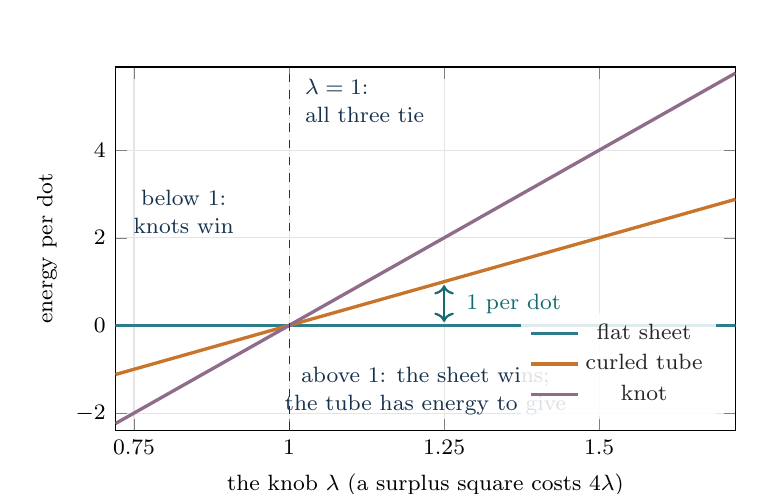
\begin{tikzpicture}
\begin{axis}[width=0.78\linewidth,height=6.2cm,xlabel={the knob $\lambda$ (a surplus square costs $4\lambda$)},ylabel={energy per dot},xmin=0.72,xmax=1.72,ymin=-2.4,ymax=5.9,xtick={0.75,1,1.25,1.5},ytick={-2,0,2,4},grid=both,grid style={gray!20},legend style={at={(0.97,0.04)},anchor=south east,font=\footnotesize,draw=none,fill=white,fill opacity=0.85},tick label style={font=\footnotesize},label style={font=\footnotesize},every axis plot/.append style={very thick}]
\addplot[flat,domain=0.72:1.72] {0};
\addplot[curl,domain=0.72:1.72] {4*(x-1)};
\addplot[melt,domain=0.72:1.72] {8*(x-1)};
\legend{flat sheet,curled tube,knot}
\draw[dashed,ink] (axis cs:1,-2.4) -- (axis cs:1,5.9);
\node[font=\footnotesize,text=ink,align=left,anchor=south west] at (axis cs:1.01,4.4) {$\lambda=1$:\\all three tie};
\node[font=\footnotesize,text=ink,align=center] at (axis cs:0.83,2.6) {below 1:\\knots win};
\node[font=\footnotesize,text=ink,align=center] at (axis cs:1.22,-1.5) {above 1: the sheet wins;\\the tube has energy to give};
\draw[<->,thick,accent] (axis cs:1.25,0.08) -- (axis cs:1.25,0.92);
\node[font=\footnotesize,text=accent,anchor=west] at (axis cs:1.27,0.5) {1 per dot};
\end{axis}
\end{tikzpicture}
\caption{The ladder against the knob. \Exact\ Each line is one rung's energy per dot as the surplus
price changes. At $\lambda=1$, the published setting, the three rungs cost the same, so turning one
into another releases nothing. Above 1 the sheet is lowest and the tube sits above it with a known
amount to give: at $\lambda=1.25$, exactly one unit per dot. Below 1 the ladder flips and a sheet
would gain by curling into knots, which is why the network breaks into knots when the surplus price is
off.}
\label{fig:ladder}
\end{figure}

This is the first thing the toy teaches. \Exact\ At the curvature setting, curled and flat cost the
same, so a curled arrangement has nothing to give and no reason to open. For a change of this kind to
happen anywhere in this family of rules, the knob has to sit above 1. There, a tube that opens into a
flat sheet gives off exactly $4(\lambda-1)$ units per dot.

That release is what the rest of this paper is about, so it gets a name of its own. The author calls
it \textbf{the burp}: the energy given off, and by extension the event that gives it off, a quiet wait,
a start, a spreading change and a definite release.

\Pub\ The standard account of a stable-for-now state giving way calls its central calculation ``the
bounce''~\cite{C77}. The two names point at opposite ends of the event. The bounce is about the start:
it gives how often a seed of the new state appears, in a quantum system that tunnels \emph{through}
its hill. The burp is about the end: what comes out. And the toy has no tunneling. Its tube goes
\emph{over} the rim, with energy lent by the bath or handed to it as a push, never through it.

\Ours\ The author reads the extra price as a \emph{curling cost}: the rule is still curvature, plus a
charge on every tightly curled link, and that charge is exactly what a burp gives back. Where space is
smooth nothing is curled tight, so the charge vanishes and only curvature remains. That reading is
hers, and it is unreviewed.

\sub{Stable for now: is there a window?}
Energy to give is not enough. Supercooled water has energy to give and sits there. For the tube to be
a stand-in for X it must be stuck: every single swap away from it must cost energy. \Exact\ At 18 dots
the model is small enough to list every allowed arrangement: there are 26, counting arrangements that
differ only in the names of their dots as one. Among them, arrangements above the flat sheet from
which every single swap costs energy exist for knob settings between 1 and 1.6, and for no larger
setting. So the knob has a window, and a narrow one.

\sub{The stand-in}
Our stand-in for X is therefore the tube. At $\lambda = 1.25$ it sits exactly one unit per dot above
the flat sheet. It is a stand-in and not X: it has one large direction where space has three, its
curled direction is always four dots around, and it lives in a network of a few hundred dots. What it
shares with X is the shape of the idea under test: a specific, curled, stable-for-now arrangement with
energy to give.

\begin{figure}[H]
\centering
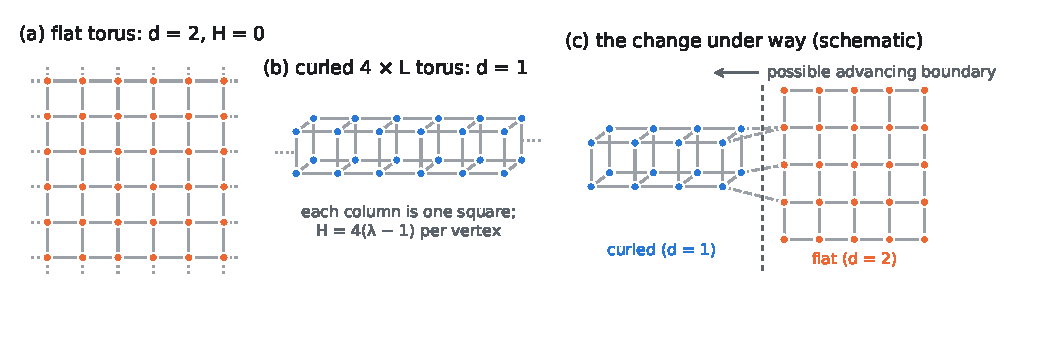
\includegraphics[width=0.96\linewidth]{fig_tori.pdf}
\caption{The two arrangements. (a) The flat sheet: a wrapping grid, two squares on every link. (b) The
$4\times L$ torus drawn as a tube: its short way around is a single square, so the links around each
column carry three. (c) A sketch of the change, not a snapshot from a simulation. In the labels, $H$
is the energy and a vertex is a dot. Spherical cows being unavailable, every space in this paper is a
torus; still, every bull burps.}
\label{fig:tori}
\end{figure}

\sub{The running example}
Take a tube of 96 dots: four around, 24 along. At $\lambda = 1.25$ it holds 96 units above the flat
sheet. That is the burp on offer. We will follow this tube through the rest of the paper so that the
amounts stay concrete. It is a running example, not an invented history: the evidence comes from
hundreds of repeated runs and, where possible, from counting every allowed move.

Now the question that decides whether any of this is a story at all. Ninety-six units are waiting to
come out. What does it cost to start?

\takeaway{A direction, in the model, is a pair of links at a dot that closes no square. Curling a
direction four steps around turns the walk around it into a square, which puts a surplus square on its
links. The tube has one large direction where the sheet has two, and sits $4(\lambda-1)$ per dot above
it: one unit per dot at $\lambda=1.25$. At $\lambda=1$ there is nothing to release, which is why the
knob sits above 1, and why this is a cousin of the published model and not the model.}

\chapterpage{4 \enspace THE OBSTACLE}{What does it cost to start?}

Before any number, consider what the number could mean. If the push needed were tiny, a few units,
then any warmth at all would set the tube off, and it would not be stable for now. If the push were
as large as the burp itself, 96 units for our tube and more for a bigger one, then starting the
change would cost what the change gives back, and the cost would grow with the size of the tube.
Nothing small could ever start something large. A sharp change of the kind pictured in Chapter~1
needs a middle answer: a push that is small, and that does not grow with the size of the thing being
pushed, so that a bigger tube releases a bigger burp from the same spark. A fixed push and a growing
release is the condition for a runaway.

So: is the cheapest exit from a perfect tube small, fixed, or neither?

\sub{Pricing the cheapest exit}
\Exact\ Start from a perfect tube and try every swap the rules allow, the one move of Chapter~2. Each
one breaks some squares and removes some surplus, and the price list gives its cost. Most are
expensive. Some cost nothing: they twist the tube around itself without changing any dot's
neighborhood, so they do not count as leaving. Among the swaps that do leave, two kinds are cheapest.
Call them route A and route B. Here are their bills at $\lambda = 1.25$, where a surplus square costs 5:

\begin{center}
\renewcommand{\arraystretch}{1.2}
\begin{tabular}{lrr}
\toprule
 & Route A & Route B \\
\midrule
Squares broken & 2 & 4 \\
\quad charged, at 16 each & $+32$ & $+64$ \\
Surplus squares removed & 4 & 10 \\
\quad refunded, at 5 each & $-20$ & $-50$ \\
\midrule
\textbf{The bill} & \textbf{12} & \textbf{14} \\
\bottomrule
\end{tabular}
\end{center}

Route A is the cheaper at this setting; the two tie at $\lambda = 4/3$, and B is the cheaper beyond.
(For readers who want every exit listed with its formula, the technical paper~\cite{tech} has them in
Section~II.)

\begin{center}
{\color{ink}\LARGE\bfseries The cheapest way out of the tube costs 12 units.}
\end{center}

Twelve. Not 96, and not 2. For our 96-dot tube the push is an eighth of what comes out; for a
288-dot tube, which holds 288 units, the same 12 is a twenty-fourth. \Exact\ The cost of the cheapest
single swap does not depend on how long the tube is, because a swap only touches a handful of
neighboring dots; the burp does, because every dot contributes one unit. That is the middle answer
the change needed, and it is arithmetic.

\begin{figure}[H]
\centering
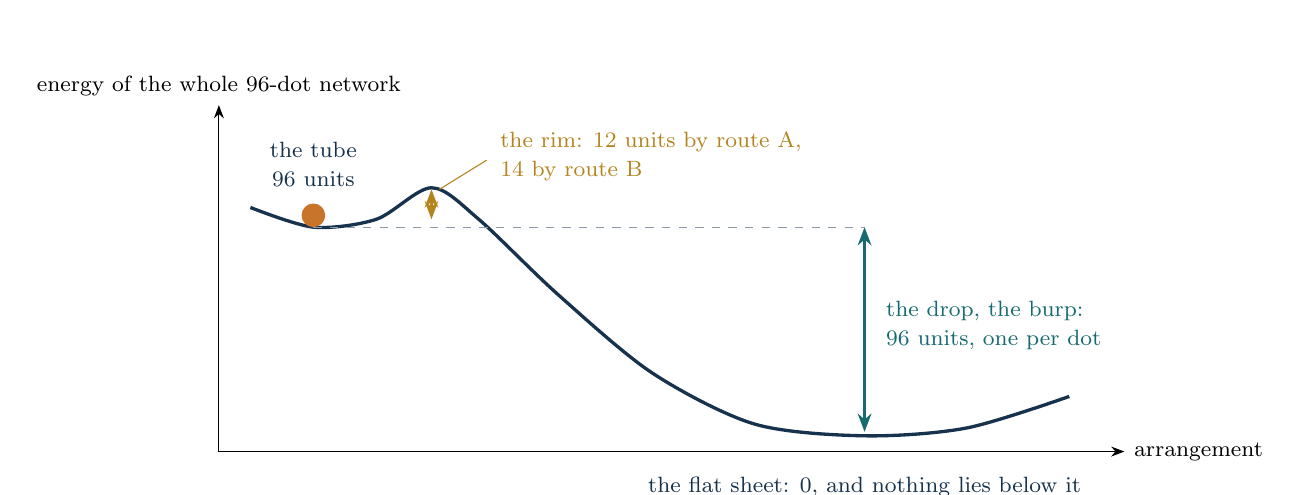
\begin{tikzpicture}[x=1cm,y=1cm,>=Stealth,font=\small]
\draw[->] (0,0) -- (0,4.4) node[above,font=\footnotesize] {energy of the whole 96-dot network};
\draw[->] (0,0) -- (11.5,0) node[right,font=\footnotesize] {arrangement};
\draw[very thick,ink] plot[smooth] coordinates {(0.4,3.1) (1.2,2.85) (2.0,2.95) (2.7,3.35) (3.3,2.95) (4.3,2.0) (5.5,1.0) (6.8,0.35) (8.2,0.2) (9.5,0.3) (10.8,0.7)};
\fill[curl] (1.2,3.0) circle (0.15);
\node[font=\footnotesize,text=ink,align=center] at (1.2,3.65) {the tube\\96 units};
\draw[<->,thick,sun!80!black] (2.7,2.95) -- (2.7,3.33);
\draw[sun!80!black] (2.8,3.33) -- (3.4,3.7);
\node[font=\footnotesize,text=sun!80!black,anchor=west,align=left] at (3.45,3.75) {the rim: 12 units by route A,\\14 by route B};
\draw[<->,thick,accent] (8.2,0.25) -- (8.2,2.85);
\node[font=\footnotesize,text=accent,anchor=west,align=left] at (8.35,1.6) {the drop, the burp:\\96 units, one per dot};
\draw[dashed,ink!50] (1.2,2.85) -- (8.2,2.85);
\node[font=\footnotesize,text=ink,align=center] at (8.2,-0.45) {the flat sheet: 0, and nothing lies below it};
\end{tikzpicture}
\caption{The landscape with its numbers filled in. \Exact\ The hollow is the tube; the rim is the
cheapest swap out; the floor is the flat sheet. For our running example the rim is 12 and the drop is
96. Make the tube three times longer and the rim is still 12 while the drop is 288.}
\end{figure}

\sub{Is 12 really the floor?}
One cheap exit from the perfect tube is not the same as no cheaper exit anywhere nearby. The free
twists lead to other arrangements with the same energy, and one of those might have a cheaper door.
\Exact\ So the calculation followed every free twist, at six sizes from 48 to 288 dots, until no new
arrangement appeared. At each size there are exactly three reachable arrangements, counting
arrangements that differ only in the names of their dots as one; every one has the same menu of exits,
and the cheapest costs 12. This is a complete finite computation, conditional on the enumeration code
being right, not a proof for every conceivable size: at a control size of 32 dots the pattern is
different, which is a reminder not to extrapolate.

\sub{The test from the other side}
Arithmetic says nothing below 12 can leave. Does 12 suffice? To find out, take the bath away and hand
the tube an exact budget and nothing more (Figure~\ref{fig:sealed}), a standard way to simulate at a
fixed total energy~\cite{Creutz83}.

\begin{figure}[H]
\centering
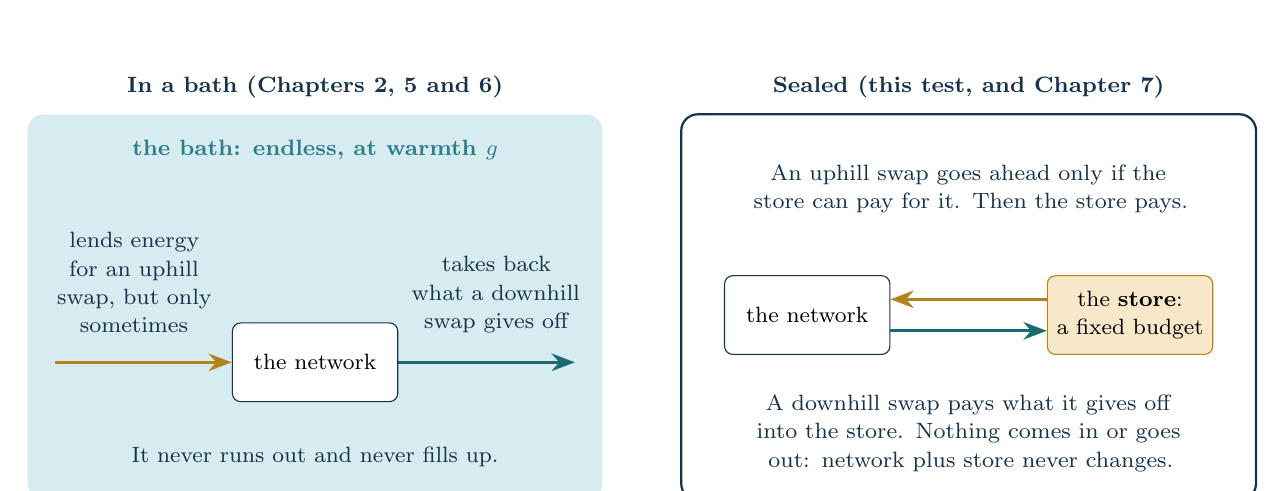
\begin{tikzpicture}[x=1cm,y=1cm,font=\footnotesize,>=Stealth]
% left: in a bath
\begin{scope}
 \fill[flatpale,rounded corners=6pt] (0,0) rectangle (7.3,4.9);
 \node[font=\footnotesize\bfseries,text=ink] at (3.65,5.25) {In a bath (Chapters 2, 5 and 6)};
 \node[text=flat,font=\footnotesize\bfseries] at (3.65,4.45) {the bath: endless, at warmth $g$};
 \node[draw=ink,fill=white,rounded corners=3pt,minimum width=2.1cm,minimum height=1.0cm] (na) at (3.65,1.75) {the network};
 \draw[->,very thick,sun!80!black] (0.35,1.75) -- (na.west);
 \draw[->,very thick,accent] (na.east) -- (6.95,1.75);
 \node[text=ink,align=center,text width=2.3cm,anchor=south] at (1.35,2.0) {lends energy for an uphill swap, but only sometimes};
 \node[text=ink,align=center,text width=2.3cm,anchor=south] at (5.95,2.0) {takes back what a downhill swap gives off};
 \node[text=ink] at (3.65,0.55) {It never runs out and never fills up.};
\end{scope}
% right: sealed
\begin{scope}[shift={(8.3,0)}]
 \draw[ink,thick,rounded corners=6pt] (0,0) rectangle (7.3,4.9);
 \node[font=\footnotesize\bfseries,text=ink] at (3.65,5.25) {Sealed (this test, and Chapter 7)};
 \node[draw=ink,fill=white,rounded corners=3pt,minimum width=2.1cm,minimum height=1.0cm] (nb) at (1.6,2.35) {the network};
 \node[draw=sun!80!black,fill=sun!25,rounded corners=3pt,minimum width=2.1cm,minimum height=1.0cm,align=center] (st) at (5.7,2.35) {the \textbf{store}:\\a fixed budget};
 \draw[->,very thick,sun!80!black] ([yshift=0.2cm]st.west) -- ([yshift=0.2cm]nb.east);
 \draw[->,very thick,accent] ([yshift=-0.2cm]nb.east) -- ([yshift=-0.2cm]st.west);
 \node[text=ink,align=center,text width=6.4cm] at (3.65,3.95) {An uphill swap goes ahead only if the store can pay for it. Then the store pays.};
 \node[text=ink,align=center,text width=6.4cm] at (3.65,0.85) {A downhill swap pays what it gives off into the store. Nothing comes in or goes out: network plus store never changes.};
\end{scope}
\end{tikzpicture}
\caption{Two ways to run the toy. \Exact\ In a bath, energy for an uphill swap is always on offer, at a
price in probability. \textbf{Sealed}, the network can spend only what its store holds. The store is
not attached to any one place: it can pay for a swap anywhere in the network, so the push is a total
budget, not a match held to one spot.}
\label{fig:sealed}
\end{figure}

\MeasX\ Try budgets of 4, 8, 10, 11, 11.5, 12, 13 and 16 units, eight runs at each budget at each of
five sizes from 48 to 192 dots: 320 runs in all, each 12,000 sweeps long.

\begin{figure}[H]
\centering
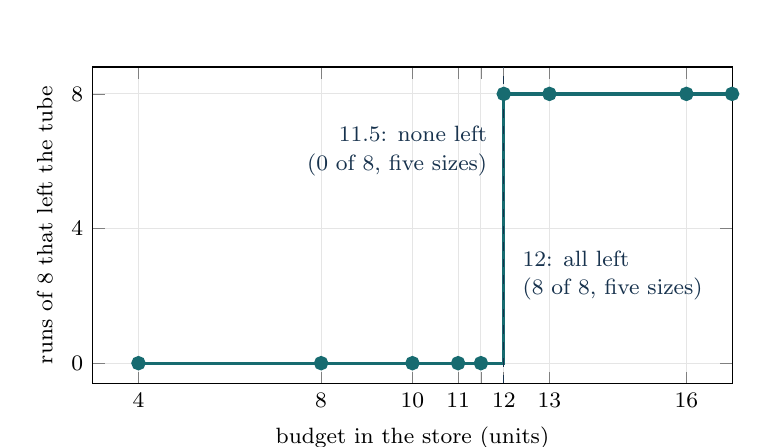
\begin{tikzpicture}
\begin{axis}[width=0.8\linewidth,height=5.6cm,xlabel={budget in the store (units)},ylabel={runs of 8 that left the tube},xmin=3,xmax=17,ymin=-0.6,ymax=8.8,xtick={4,8,10,11,11.5,12,13,16},xticklabels={4,8,10,11,{},12,13,16},ytick={0,4,8},grid=both,grid style={gray!20},tick label style={font=\footnotesize},label style={font=\footnotesize}]
\addplot[accent,very thick,const plot mark left,mark=*,mark options={fill=accent}] coordinates {(4,0) (8,0) (10,0) (11,0) (11.5,0) (12,8) (13,8) (16,8) (17,8)};
\draw[dashed,ink] (axis cs:12,-0.6) -- (axis cs:12,8.8);
\node[font=\footnotesize,text=ink,anchor=east,align=right] at (axis cs:11.85,6.3) {11.5: none left\\(0 of 8, five sizes)};
\node[font=\footnotesize,text=ink,anchor=west,align=left] at (axis cs:12.2,2.6) {12: all left\\(8 of 8, five sizes)};
\end{axis}
\end{tikzpicture}
\caption{The staircase. \MeasX\ The same curve at all five sizes, 48 to 192 dots: every budget below
12 gave zero escapes, every budget of 12 or more gave eight of eight. Pooled over the sizes, none of
200 runs left with a budget below 12, and all 120 left with 12 or more. The flag counted
\emph{leaving} the tube, not finishing the change.}
\label{fig:staircase}
\end{figure}

\Exact\ The lower half of this staircase is a theorem of the model at these sizes: with no exit
cheaper than 12 and a store that cannot go negative, a budget below 12 can only pay for free twists.
The upper half is an observation about this protocol and duration.\footnote{Why not run a hundred
tubes at each budget instead of eight? Our reasoning, from the exact counts, is that it would add
little. Below 12, leaving is impossible, which is
arithmetic, and no number of runs can strengthen it. At 12 or more, the count of Chapter~5 says a
perfect tube is offered, on average, three exits costing 12 in every sweep, and with 12 in the store
the first one offered is paid for at once. A run that stayed put for 12,000 sweeps would itself be
the surprise. The runs check that count; they are not estimating an unknown chance.}
\MeasX\ Together they say that the wall is local, exactly 12 units high at $\lambda=1.25$, and the same
at every size tried, while what waits behind it grows with the system.

\whyhere{This is the pivot of the whole paper. Suppose the push had grown with the size of the tube,
so that a tube twice as long needed a push twice as large. Then no single spot could start the change:
something would have to push the whole tube at once, and the picture of a seed and a spreading front
would fail in this model. We would have had to look for this kind of change in another one. A fixed,
cheap push against a growing release is the condition under which something small can start something
large.}

\takeaway{Twelve units: the cost of the cheapest partner swap out of a perfect tube, counted exactly,
the same at every size, and confirmed from the other side by 320 sealed runs. The release grows with
the tube; the push does not.}

\chapterpage{5 \enspace THE WAIT}{How long before the door opens, and what kind of waiting is it?}

A rim of 12 says what a push must be. It does not say when a tube left to itself will go. For that we
put it back in the bath of Chapter~2 and let the network jiggle at warmth $g$. A swap that climbs the
rim, costing 12, is accepted with chance $e^{-12/g}$: warmer, and the rim is cleared more often.

\sub{A lottery with counted tickets}
Now the wait becomes a lottery, and every ticket can be counted. \Exact\ In one sweep the computer
proposes two swaps for every dot, $2N$ in all for a tube of $N$ dots, each one picked at random from
every swap there is. How many of those proposals are exits?

Take route A. A tube of $N$ dots has $3N$ different route-A swaps: three for every dot, so a longer
tube has more ways out. But a longer tube also has more swaps of every other kind, and those grow
faster, as $N$ times $N$. So the chance that any one proposal lands on a route-A exit is 3 in $2N$,
smaller for a longer tube. A sweep makes $2N$ proposals. Multiply the two and the length cancels:
\[
2N \;\times\; \frac{3}{2N} \;=\; 3 .
\]
A sweep offers three route-A exits on average, whatever the size of the tube. A longer tube has more
exits, each one is harder to hit, and with two proposals per dot in a sweep the two effects balance
exactly. The same count for route B gives two.

Each offer of A is accepted with chance $e^{-12/g}$, each offer of B with chance $e^{-14/g}$. So the
chance of leaving in any one sweep is $3\,e^{-12/g} + 2\,e^{-14/g}$, and the mean wait is one divided
by that, with nothing fitted:
\[
\text{mean wait} \;=\; \frac{1}{3\,e^{-12/g} + 2\,e^{-14/g}} \quad\text{sweeps.}
\]
At $g = 1.5$, the warmth used for most runs below, that is 845 sweeps. Chemists know this shape as an
Arrhenius law. Here both of its ingredients, the height of the rim and the number of tries per sweep,
are counted from the arrangement rather than fitted to the data (the technical paper~\cite{tech},
Section~II, gives the formula for any $\lambda$).

\begin{figure}[H]
\centering
\resizebox{\linewidth}{!}{%
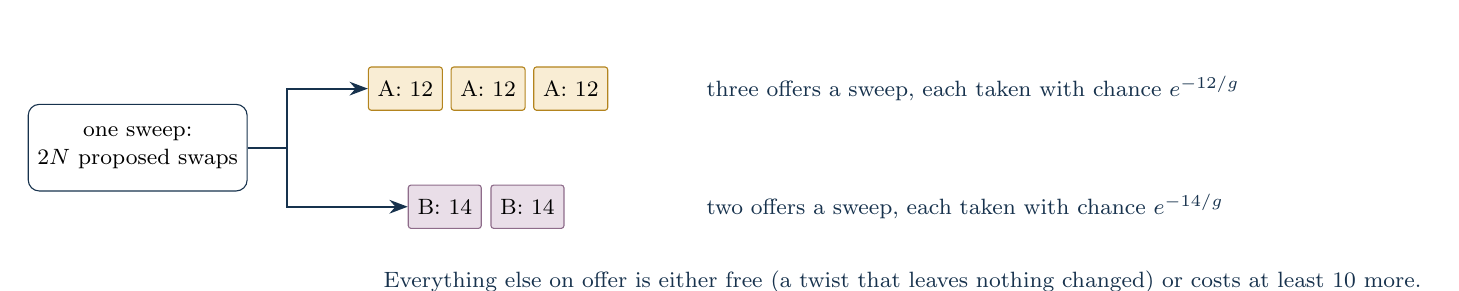
\begin{tikzpicture}[x=1cm,y=1cm,font=\small,>=Stealth]
\node[draw=ink,rounded corners,minimum width=2.6cm,minimum height=1.1cm,align=center,font=\footnotesize] (sw) at (0,0) {one sweep:\\$2N$ proposed swaps};
\foreach \i in {0,1,2} {\node[draw=sun!80!black,fill=sun!20,rounded corners=1pt,minimum width=0.9cm,minimum height=0.55cm,font=\footnotesize] (a\i) at (3.4+\i*1.05,0.75) {A: 12};}
\foreach \i in {0,1} {\node[draw=melt,fill=meltpale,rounded corners=1pt,minimum width=0.9cm,minimum height=0.55cm,font=\footnotesize] (b\i) at (3.9+\i*1.05,-0.75) {B: 14};}
\draw[->,thick,ink] (sw.east) -- ++(0.5,0) |- (a0.west);
\draw[->,thick,ink] (sw.east) -- ++(0.5,0) |- (b0.west);
\node[font=\footnotesize,text=ink,anchor=west,align=left] at (7.1,0.75) {three offers a sweep, each taken with chance $e^{-12/g}$};
\node[font=\footnotesize,text=ink,anchor=west,align=left] at (7.1,-0.75) {two offers a sweep, each taken with chance $e^{-14/g}$};
\node[font=\footnotesize,text=ink,anchor=west,align=left] at (3.0,-1.7) {Everything else on offer is either free (a twist that leaves nothing changed) or costs at least 10 more.};
\end{tikzpicture}}
\caption{The lottery. \Exact\ The tickets are counted, not estimated: the perfect tube offers, on
average, exactly three route-A exits and two route-B exits per sweep whatever its length. The chance of each being
taken is set by the bath's warmth $g$.}
\end{figure}

\sub{Does the tube keep the appointment?}
\MeasX\ The first test ran twelve conditions at $\lambda = 1.25$: six warmths from $g=1.4$ to 2.5, two
sizes, sixteen tubes each, with measured waits from about 30 sweeps to about 2,500. The prediction
written down for this test counted route A only, which makes the predicted wait a little longer than
the full formula does: 994 sweeps at $g=1.5$, where the full formula gives 845.

Averaged over the twelve conditions, the measured wait came within 2 percent of the predicted one.
One condition at a time the match is looser: they range from 29 percent shorter than predicted to 62
percent longer (Figure~\ref{fig:twelve}). That is the scatter a lottery gives: with only sixteen tubes,
their average wait lands, by chance alone, about 25 percent above or below the true average. The two sizes
also differ. The 144-dot tubes sit near the full formula, and the 64-dot tubes waited longer. This
exploratory test cannot say whether that is chance, which is one reason for the stricter test below.

\begin{figure}[H]
\centering
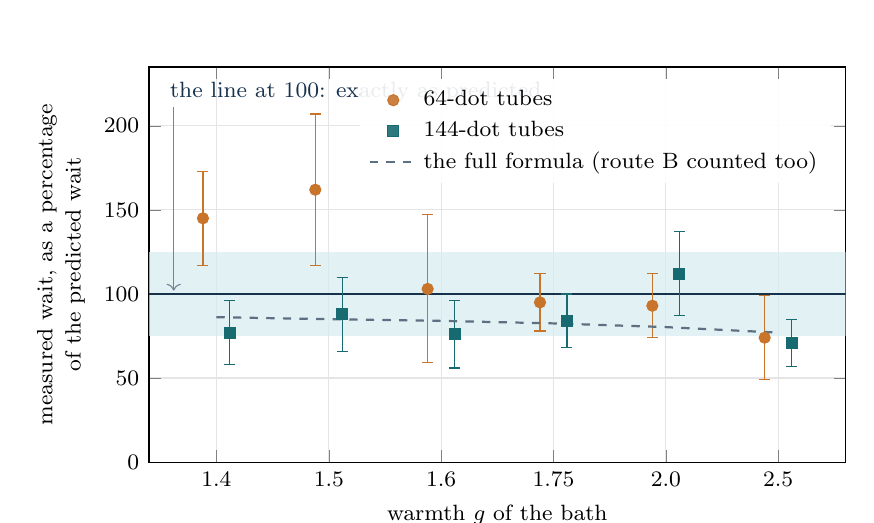
\begin{tikzpicture}
\begin{axis}[width=0.86\linewidth,height=6.6cm,xlabel={warmth $g$ of the bath},ylabel={measured wait, as a percentage\\of the predicted wait},ylabel style={align=center},xmin=0.4,xmax=6.6,ymin=0,ymax=235,xtick={1,2,3,4,5,6},xticklabels={1.4,1.5,1.6,1.75,2.0,2.5},ytick={0,50,100,150,200},grid=both,grid style={gray!20},tick label style={font=\footnotesize},label style={font=\footnotesize},legend style={at={(0.98,0.97)},anchor=north east,font=\footnotesize,draw=none,fill=white,fill opacity=0.9,text opacity=1},legend cell align=left]
\fill[flatpale,opacity=0.7] (axis cs:0.4,75) rectangle (axis cs:6.6,125);
\draw[ink,thick] (axis cs:0.4,100) -- (axis cs:6.6,100);
\addplot[curl,only marks,mark=*,mark options={fill=curl},error bars/.cd,y dir=both,y explicit] coordinates {(0.88,145) +- (0,28) (1.88,162) +- (0,45) (2.88,103) +- (0,44) (3.88,95) +- (0,17) (4.88,93) +- (0,19) (5.88,74) +- (0,25)};
\addplot[accent,only marks,mark=square*,mark options={fill=accent},error bars/.cd,y dir=both,y explicit] coordinates {(1.12,77) +- (0,19) (2.12,88) +- (0,22) (3.12,76) +- (0,20) (4.12,84) +- (0,16) (5.12,112) +- (0,25) (6.12,71) +- (0,14)};
\addplot[ink!70,dashed,thick] coordinates {(1,86.2) (2,85.0) (3,84.0) (4,82.5) (5,80.3) (6,77.0)};
\legend{64-dot tubes,144-dot tubes,the full formula (route B counted too)}
\node[font=\footnotesize,text=ink,anchor=west] (lab) at (axis cs:0.5,220) {the line at 100: exactly as predicted};
\draw[ink!60,->] (axis cs:0.62,211) -- (axis cs:0.62,102);
\end{axis}
\end{tikzpicture}
\caption{Twelve conditions against the count. \MeasX\ Each mark is the average wait of sixteen tubes,
shown as a percentage of the wait predicted from route A alone, so 100 means exactly as predicted. The
bar through a mark is its uncertainty. The shaded band, 25 percent either way, is where such an average
usually lands by chance when the prediction is right. The dashed line is where the full formula, with
route B counted too, puts the prediction.}
\label{fig:twelve}
\end{figure}

\Meas\ A stricter, pre-registered test then counted every single accepted swap in 240 further runs
across six settings of $\lambda$ and size, and compared the first exits with the full formula, both
routes. All 240 first exits were observed, and their mean arrived when the formula said it would in
every cell, within the scatter expected from that many runs.

\begin{figure}[H]
\centering
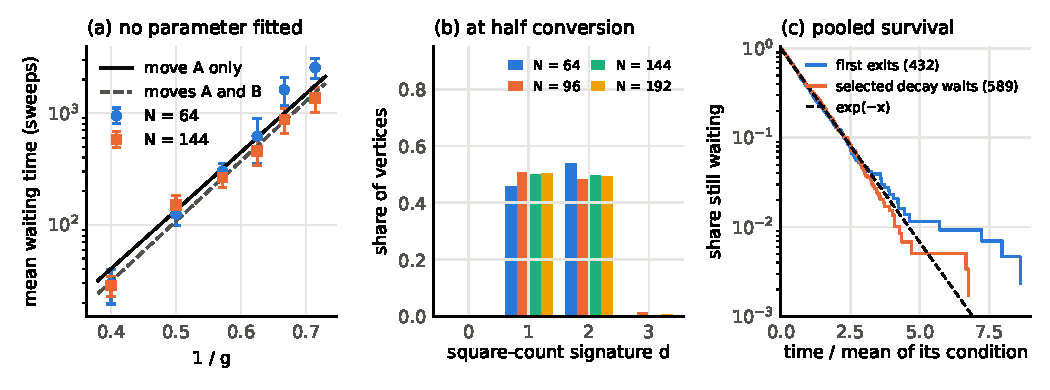
\includegraphics[width=\linewidth]{fig1.pdf}
\caption{The wait, measured. (a) Mean waiting time against the inverse warmth $1/g$, at
$\lambda=1.25$; the lines are the formula with route A alone (solid) and A plus B (dashed), nothing
fitted. (b) The share of dots at each direction count $d$ halfway through the change, averaged over
thirty runs per size: almost everything is at 1 or 2. (c) The fraction of tubes still waiting against
time, in units of each condition's mean; a memoryless wait gives the dashed straight line.}
\end{figure}

\sub{What kind of waiting}
If the chance of escape is the same on every attempt, the waits are \textbf{memoryless}. It is like
rolling a die until a six comes up: twenty rolls without one do not make a six any likelier on the next
roll, and a tube that has waited a long time is no nearer to leaving. One sign of a memoryless wait is
that the waits spread out by about as much as their average. \Meas\ That check was pre-registered, and
it passed at every size in the main run. \MeasX\ Checked afterwards, the whole distribution of first exits is consistent with that
picture too, panel (c) above. The time to a \emph{detected} change looked different, with a tail the
first exits do not have. Chapter~9 finds out why.

\Meas\ One more thing the move-by-move count revealed: the first swap out does not always lead
anywhere. Think of that first swap as a door opening. About a third of the time the door closes again,
and the tube goes back to being a perfect tube. Only 56 to 68 percent of first exits went on to a real
change, with no trend in $\lambda$. The formula predicts when the door opens, not the departure.

\sub{A caution about the clock}
\Ours\ The clock here counts attempted swaps, not seconds. One sweep offers any one neighborhood a
way out about $1/N$ as often as a clock that gave every neighborhood its own fixed rate would. On that
fairer clock the wait would fall as $1/N$, and a longer tube would go sooner. The model has no time
in it; which clock is ``right'' is not a question it can answer, and a later paper adopts the
fairer one.

\whyhere{If the measured wait had disagreed with the counted lottery, something larger than a single
swap would be holding the tube shut, and 12 would have been the wrong number. It agrees. The rim is the
single swap, and the lottery is the whole explanation of the first exit.}

\takeaway{Count the exits a sweep offers, multiply by the chance each is taken, and you predict the
mean wait with nothing fitted. The tube keeps that appointment over a ninety-fold range of waits, and
its waiting is memoryless, like rolling for a six. But about a third of the time the door closes
again: an opened door is not a departure.}

\chapterpage{6 \enspace THE CHANGE}{What takes shape on the other side}

Chapter~5 was about the start: the first swap out, and whether it holds. This chapter is about what
comes next: how the change spreads through the tube. It spreads fast.

The natural picture is a zipper. One spot of the tube opens, and the opening runs along the tube the
way a zipper runs along a jacket. The slider, the tab you pull, is the boundary: behind it the tube
has already opened into flat sheet, and ahead of it the tube is still closed. Physicists call a moving
boundary like this a \textbf{front}. To find out whether the zipper picture is right, we need an
instrument.

\Exact\ The fastest instrument is the direction count $d$ of Chapter~3. Dots still in the tube read
$d = 1$; dots on a flat sheet read $d = 2$; a melted, disordered dot reads 0 or 3 and up. The program
marks every dot and also keeps a progress meter that runs from 0 (all tube) to 1 (all flat). It takes
a snapshot of the whole network at three stages fixed in advance: when the meter first reads a
quarter, a half and three-quarters. These are stages of the change, not times on the clock, and there
is nothing special about them. They were fixed beforehand so that nobody could pick a moment because
its picture looks persuasive. The predictions were scored at the half mark, where tube and sheet are
most evenly matched and anything in between would have the most room to show.

\Meas\ At $\lambda = 1.25$ and $g=1.5$, thirty tubes at each of four sizes, run twice with fresh random
numbers, and three predictions written down first: a memoryless wait; at least 80 percent of dots in
one of the two signatures at the half mark; and at least 70 percent of the flat-like dots in one
connected region, on average. All three held at every size in both runs. At the half mark 98.8 to 99.8
percent of dots read as tube or sheet. The other two snapshots were recorded but not scored. Read
afterwards, they say the same: 98.8 to 99.7 percent at a quarter, and 98.5 to 99.5 percent at
three-quarters. Something organized was happening, early, midway and late, with almost nothing in
between.

\begin{figure}[H]
\centering
\resizebox{\linewidth}{!}{%
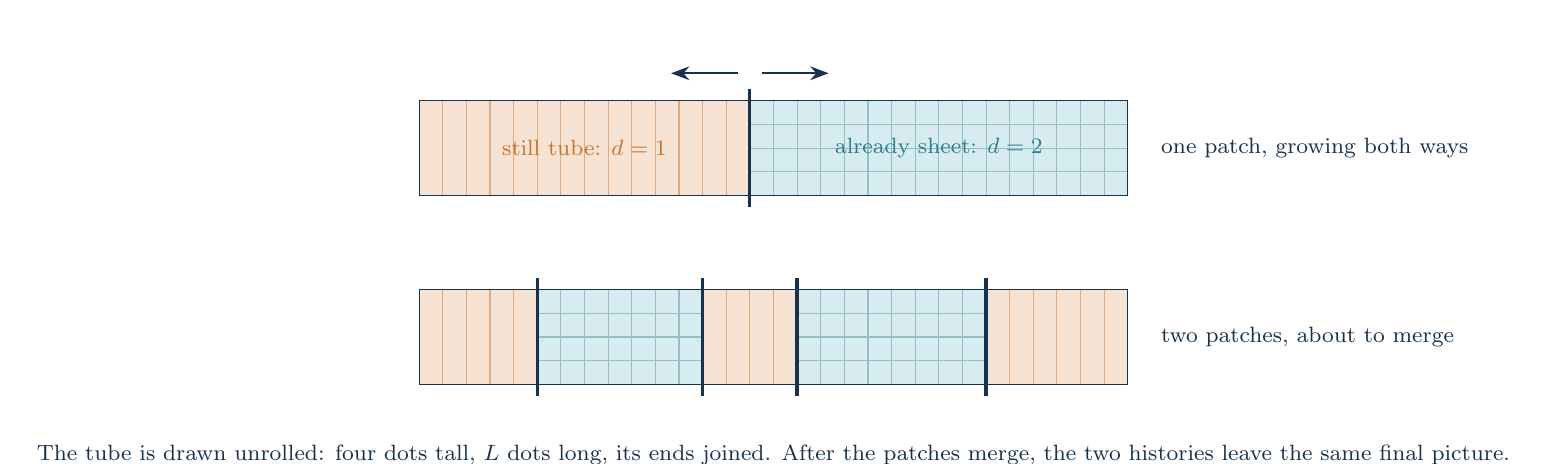
\begin{tikzpicture}[x=1cm,y=1cm,font=\small,>=Stealth]
% unrolled tube, one front
\begin{scope}
\fill[curlpale] (0,0) rectangle (4.2,1.2);
\foreach \x in {0.3,0.6,...,4.0} {\draw[curl!60] (\x,0) -- (\x,1.2);}
\fill[flatpale] (4.2,0) rectangle (9.0,1.2);
\draw[flat!50,step=0.3] (4.2,0) grid (9.0,1.2);
\draw[ink] (0,0) rectangle (9,1.2);
\draw[very thick,ink] (4.2,-0.15) -- (4.2,1.35);
\draw[->,thick,ink] (4.35,1.55) -- (5.2,1.55);
\draw[->,thick,ink] (4.05,1.55) -- (3.2,1.55);
\node[font=\footnotesize,text=curl] at (2.1,0.6) {still tube: $d=1$};
\node[font=\footnotesize,text=flat] at (6.6,0.6) {already sheet: $d=2$};
\node[font=\footnotesize,text=ink,anchor=west] at (9.3,0.6) {one patch, growing both ways};
\end{scope}
% two patches
\begin{scope}[shift={(0,-2.4)}]
\fill[curlpale] (0,0) rectangle (9,1.2);
\foreach \x in {0.3,0.6,...,8.8} {\draw[curl!60] (\x,0) -- (\x,1.2);}
\fill[flatpale] (1.5,0) rectangle (3.6,1.2); \draw[flat!50,step=0.3] (1.5,0) grid (3.6,1.2);
\fill[flatpale] (4.8,0) rectangle (7.2,1.2); \draw[flat!50,step=0.3] (4.8,0) grid (7.2,1.2);
\draw[ink] (0,0) rectangle (9,1.2);
\foreach \x in {1.5,3.6,4.8,7.2} {\draw[very thick,ink] (\x,-0.15) -- (\x,1.35);}
\node[font=\footnotesize,text=ink,anchor=west] at (9.3,0.6) {two patches, about to merge};
\end{scope}
\node[font=\footnotesize,text=ink,align=center] at (4.5,-3.3) {The tube is drawn unrolled: four dots tall, $L$ dots long, its ends joined. After the patches merge, the two histories leave the same final picture.};
\end{tikzpicture}}
\caption{What ``one zipper'' can and cannot mean. \Sketch\ Both histories end with one large
connected sheet-like region, and a snapshot cannot always tell them apart. The tube is a loop, so even
a single open patch has two sliders, one at each end, moving apart.}
\label{fig:zipper}
\end{figure}

\sub{What the count cannot vouch for}
A jacket found open along one long stretch could have been unzipped from one spot, or from two spots
whose openings ran into each other before anyone looked. So one large open region is weaker evidence
than one zipper. \Meas\ The averages passed the 70-percent rule at every size, but individual runs did
not always. Of the thirty runs at 64, 96, 144 and 192 dots, 0, 2, 4 and 9 fell below it in the first
set, and 0, 1, 3 and 5 in the second. A separate pre-registered test of a simple one-front law came
out NOT ESTABLISHED: 21 of 59 tubes that started converted in several patches, mostly at the warmer
bath. The honest description is that one connected flat-like region usually dominates by the half
mark, and that the change often starts in more than one place: more than one zipper.

Nor does a count certify a geometry. \Exact\ A single swap from a perfect tube can produce dots that
read $d=2$ while their links carry one, two, two and three squares, which no dot on a flat sheet
does. Two buildings can contain the same number of rooms and have different floor plans. And a grid
six steps around and enormously long reads flat at every dot while keeping one direction short. The
paper therefore calls $d = 1$ and $d=2$ \emph{curled-like} and \emph{flat-like} signatures. When it
says the curled direction opened, it means only that the four-step curl is gone, not that both
directions were shown to grow large. The second has not been measured.

\begin{figure}[H]
\centering
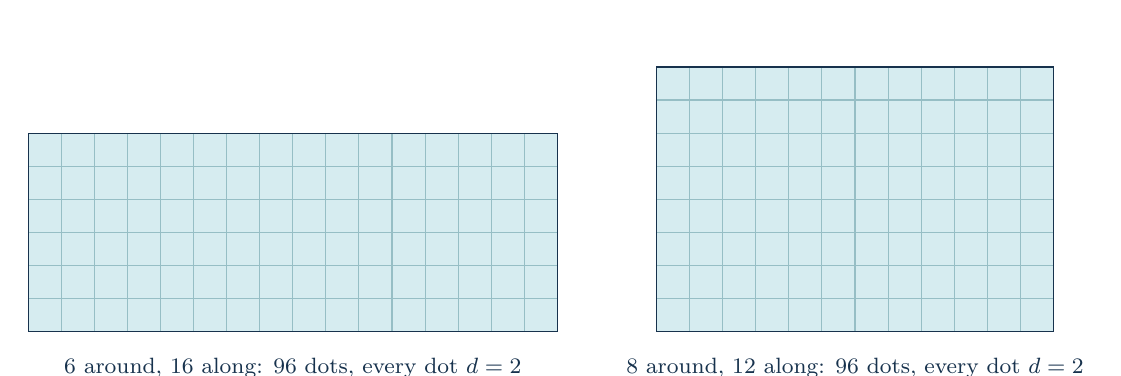
\begin{tikzpicture}[x=0.42cm,y=0.42cm,font=\small]
\begin{scope}
\fill[flatpale] (0,0) rectangle (16,6); \draw[flat!50,step=1] (0,0) grid (16,6); \draw[ink] (0,0) rectangle (16,6);
\node[font=\footnotesize,text=ink] at (8,-1.1) {6 around, 16 along: 96 dots, every dot $d=2$};
\end{scope}
\begin{scope}[shift={(19,0)}]
\fill[flatpale] (0,0) rectangle (12,8); \draw[flat!50,step=1] (0,0) grid (12,8); \draw[ink] (0,0) rectangle (12,8);
\node[font=\footnotesize,text=ink] at (6,-1.1) {8 around, 12 along: 96 dots, every dot $d=2$};
\end{scope}
\end{tikzpicture}
\caption{Same count, different floor plan. \Exact\ Both grids wrap in both directions, cost zero, and
read $d=2$ at every dot. The left one still has a short way around. The signature alone cannot tell
them apart; only measuring both ways around could.}
\end{figure}

\sub{A stronger look at the finished wiring}
\Exact\ For the 120 saved final networks at $\lambda = 1.05$, the smallest knob setting in the map of
Chapter~9, the check was done the hard way, from the wiring itself (Figure~\ref{fig:certify}). All 120
passed. Those endpoints are tori, established from the wiring and not from a count. Their two ways
around were not measured.

\begin{figure}[H]
\centering
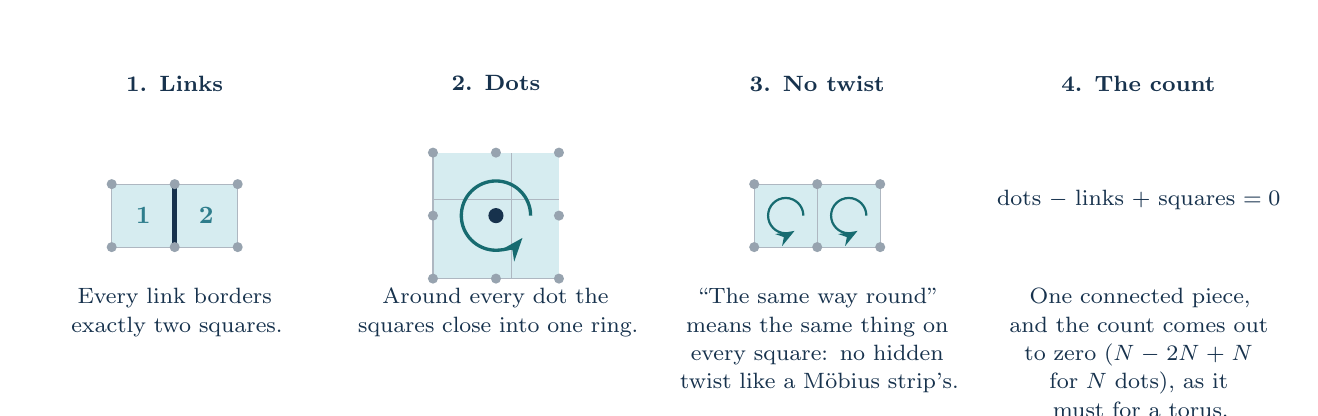
\begin{tikzpicture}[x=0.8cm,y=0.8cm,font=\footnotesize,>=Stealth]
% 1: two squares on every link
\begin{scope}
 \fill[flatpale] (0,0) rectangle (2,1);
 \draw[ink!35] (0,0) rectangle (2,1);
 \draw[line width=2pt,ink] (1,0) -- (1,1);
 \foreach \p in {(0,0),(1,0),(2,0),(0,1),(1,1),(2,1)} {\fill[ink!45] \p circle (0.08);}
 \node[text=flat,font=\small\bfseries] at (0.5,0.5) {1}; \node[text=flat,font=\small\bfseries] at (1.5,0.5) {2};
 \node[font=\footnotesize\bfseries,text=ink] at (1,2.6) {1. Links};
 \node[text=ink,align=center,text width=3.5cm,anchor=north] at (1,-0.5) {Every link borders exactly two squares.};
\end{scope}
% 2: the squares around a dot form one ring
\begin{scope}[shift={(5.1,-0.5)}]
 \fill[flatpale] (0,0) rectangle (2,2);
 \draw[ink!35] (0,0) grid (2,2);
 \foreach \i in {0,1,2} \foreach \j in {0,1,2} {\fill[ink!45] (\i,\j) circle (0.08);}
 \fill[ink] (1,1) circle (0.12);
 \draw[->,accent,very thick] (1.55,1) arc (0:320:0.55);
 \node[font=\footnotesize\bfseries,text=ink] at (1,3.1) {2. Dots};
 \node[text=ink,align=center,text width=3.5cm,anchor=north] at (1,0.0) {Around every dot the squares close into one ring.};
\end{scope}
% 3: one sense of turning everywhere
\begin{scope}[shift={(10.2,0)}]
 \fill[flatpale] (0,0) rectangle (2,1);
 \draw[ink!35] (0,0) rectangle (2,1) (1,0) -- (1,1);
 \foreach \p in {(0,0),(1,0),(2,0),(0,1),(1,1),(2,1)} {\fill[ink!45] \p circle (0.08);}
 \draw[->,accent,thick] (0.78,0.5) arc (0:300:0.28);
 \draw[->,accent,thick] (1.78,0.5) arc (0:300:0.28);
 \node[font=\footnotesize\bfseries,text=ink] at (1,2.6) {3. No twist};
 \node[text=ink,align=center,text width=3.5cm,anchor=north] at (1,-0.5) {``The same way round'' means the same thing on every square: no hidden twist like a M\"obius strip's.};
\end{scope}
% 4: one piece, and the count
\begin{scope}[shift={(15.3,0)}]
 \node[font=\footnotesize\bfseries,text=ink] at (1,2.6) {4. The count};
 \node[text=ink,align=center,text width=3.6cm] at (1,0.75) {dots $-$ links $+$ squares $= 0$};
 \node[text=ink,align=center,text width=3.6cm,anchor=north] at (1,-0.5) {One connected piece, and the count comes out to zero ($N - 2N + N$ for $N$ dots), as it must for a torus.};
\end{scope}
\end{tikzpicture}
\caption{Certifying a torus from its wiring. \Exact\ Four checks, run on each of the 120 saved networks
after filling in every square. A network that passes all four is a torus, whatever its dots' direction
counts say.}
\label{fig:certify}
\end{figure}

\sub{The energy comes out exactly}
\Meas\ When a tube finishes as a perfect flat sheet, the energy given off is exactly one unit per dot
at $\lambda = 1.25$: the arithmetic of Chapter~3, now measured. In 24 to 28 of 30 runs per size the
release was within one percent of that. The rest settled on sheets with small defects, 8 to 45 units'
worth read from their wiring, and held back that much. The ideal gap is exact; how much of it comes
out depends on where the network stops.

\whyhere{A sharp change means two arrangements side by side with a front between them, not everything
softening at once. Only a snapshot in the middle of the change can test that, and only an instrument
fixed in advance keeps us from choosing the snapshot we like.}

\takeaway{A quarter, half and three-quarters of the way through, about 99 dots in 100 read as tube or
sheet, and one connected sheet-like region usually dominates. That is sharp in the sense written down
beforehand. It is not proof of a single zipper, and a count is not a geometry: the finished tori were certified from their wiring, and whether
both ways around grew large has not been measured.}

\chapterpage{7 \enspace CLOSE THE LID}{Where does the energy go when it has nowhere to go?}

Apart from the budget test of Chapter~4, every run so far sat in the bath, and the bath carried the
released energy away as fast as it appeared. If a change like this made all of space, there was no
outside for its energy to go to. So seal the system again, as in Chapter~4, and watch what the burp
does to its own surroundings.

\Exact\ The sealed system of Chapter~4 had one store. Here there are $C$ stores beside the network,
each holding a non-negative number of units. Every proposed swap picks one store at random: an uphill
swap is refused unless that store can pay; a downhill swap deposits its release there. Nothing enters
or leaves, so network plus stores is constant to the unit, and it was checked to be constant in every
run.

Return to our 96-dot tube, holding 96 units. Put 12 more in a store and seal the lid. The account
reads 108. Suppose the change runs and leaves one 14-unit scrap in the sheet, as Chapter~8 will show
it often does. The network has gone from 96 to 14; the stores have gone from 12 to 94.

\begin{figure}[H]
\centering
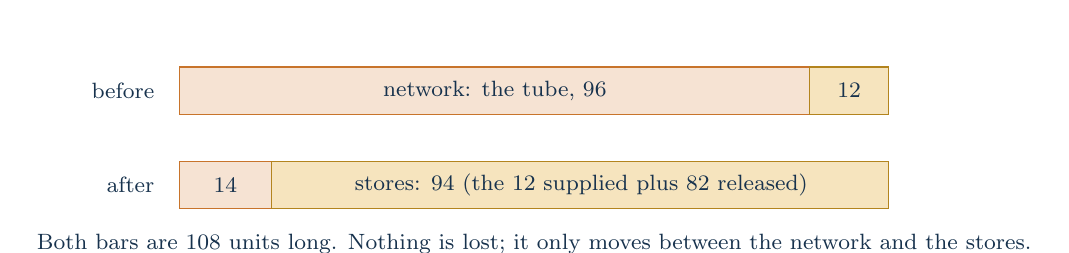
\begin{tikzpicture}[x=1cm,y=1cm,font=\small]
\node[font=\footnotesize,text=ink,anchor=east] at (-0.2,1.5) {before};
\fill[curlpale,draw=curl] (0,1.2) rectangle (8.0,1.8); \node[font=\footnotesize,text=ink] at (4.0,1.5) {network: the tube, 96};
\fill[sun!30,draw=sun!80!black] (8.0,1.2) rectangle (9.0,1.8); \node[font=\footnotesize,text=ink] at (8.5,1.5) {12};
\node[font=\footnotesize,text=ink,anchor=east] at (-0.2,0.3) {after};
\fill[curlpale,draw=curl] (0,0) rectangle (1.17,0.6); \node[font=\footnotesize,text=ink] at (0.58,0.3) {14};
\fill[sun!30,draw=sun!80!black] (1.17,0) rectangle (9.0,0.6); \node[font=\footnotesize,text=ink] at (5.1,0.3) {stores: 94 (the 12 supplied plus 82 released)};
\node[font=\footnotesize,text=ink] at (4.5,-0.45) {Both bars are 108 units long. Nothing is lost; it only moves between the network and the stores.};
\end{tikzpicture}
\caption{The ledger for the running example. \Exact\ The bookkeeping is exact in every sealed run; the
particular ending shown here, one 14-unit scrap, is an illustration of a common outcome, not a
promise about any one run.}
\end{figure}

\sub{The surroundings can spoil the ending}
Here is the twist. The released energy is now in the stores, and the stores pay for uphill swaps.
Energy that has nowhere to go can buy swaps that break the very squares the change has just made.
How much damage depends on how many stores there are. \Pub\ Many stores share the release thinly, like
a large cold room; few stores concentrate it, like a small hot one.

\Meas\ Pre-registered: tubes of 64, 96 and 192 dots, seven choices of $C$ from a single store to two per
dot, twenty runs at each setting, 420 runs. The outcomes were classified by rules fixed beforehand:
sheet-like if at least 90 percent of dots read $d=2$ with almost no melted dots; melted if 15 percent
or more read as disorder; stalled if both orders sat side by side with nothing melting; in between
otherwise.

\begin{figure}[H]
\centering
\pgfplotsset{resbar/.style={ybar stacked,bar width=9pt,width=5.0cm,height=5.0cm,ymin=0,ymax=20,ytick={0,10,20},symbolic x coords={1,N/16,N/8,N/4,N/2,N,2N},xtick=data,x tick label style={rotate=60,anchor=east,font=\scriptsize},tick label style={font=\footnotesize},label style={font=\footnotesize},enlarge x limits=0.1}}
\begin{tikzpicture}
\begin{axis}[resbar,title={64 dots},title style={font=\footnotesize},ylabel={runs of 20}]
\addplot[fill=flat,draw=none] coordinates {(1,0) (N/16,0) (N/8,0) (N/4,3) (N/2,18) (N,20) (2N,20)};
\addplot[fill=gray!45,draw=none] coordinates {(1,3) (N/16,3) (N/8,8) (N/4,13) (N/2,2) (N,0) (2N,0)};
\addplot[fill=melt,draw=none] coordinates {(1,17) (N/16,17) (N/8,12) (N/4,4) (N/2,0) (N,0) (2N,0)};
\end{axis}
\end{tikzpicture}
\begin{tikzpicture}
\begin{axis}[resbar,title={96 dots},title style={font=\footnotesize},yticklabels={}]
\addplot[fill=flat,draw=none] coordinates {(1,0) (N/16,0) (N/8,0) (N/4,1) (N/2,19) (N,19) (2N,20)};
\addplot[fill=gray!45,draw=none] coordinates {(1,2) (N/16,2) (N/8,11) (N/4,17) (N/2,1) (N,1) (2N,0)};
\addplot[fill=melt,draw=none] coordinates {(1,18) (N/16,18) (N/8,9) (N/4,2) (N/2,0) (N,0) (2N,0)};
\end{axis}
\end{tikzpicture}
\begin{tikzpicture}
\begin{axis}[resbar,title={192 dots},title style={font=\footnotesize},yticklabels={},legend style={at={(1.05,0.5)},anchor=west,font=\footnotesize,draw=none},legend cell align=left]
\addplot[fill=flat,draw=none] coordinates {(1,0) (N/16,0) (N/8,0) (N/4,0) (N/2,19) (N,20) (2N,20)};
\addplot[fill=gray!45,draw=none] coordinates {(1,0) (N/16,1) (N/8,4) (N/4,18) (N/2,1) (N,0) (2N,0)};
\addplot[fill=melt,draw=none] coordinates {(1,20) (N/16,19) (N/8,16) (N/4,2) (N/2,0) (N,0) (2N,0)};
\legend{sheet-like,in between,melted}
\end{axis}
\end{tikzpicture}
\caption{Bonfire or melt. \Meas\ The horizontal axis is the number of stores $C$, as a share of the
number of dots $N$. With few stores the release melts the new sheet back into disorder; with many it
leaves a clean sheet. The switch-over lies between one store per four dots and one per two at all
three sizes, and no run ended stalled with both orders side by side. Totals: 179 sheet-like, 87 in
between, 154 melted.}
\end{figure}

\Meas\ A bonfire with a threshold, as the pre-registered verdict put it. Where the heat has room, the
change feeds itself to completion; where it does not, the heat melts what the change made. Melted
means the dots lose their neat two directions and go back to being linked any old way, which is the
random phase the published model starts from. The switch-over moves in step with size, as a release
of one unit per dot shared among the stores predicts. \Ours\ A rough energy budget puts it near one
store per three dots; the measured crossover sits between one per four and one per two, which is as
fine as the grid can say. That estimate assumes the stores settle into a thermal balance, and
individual store balances were not saved, so it is a budget, not a calibrated thermometer.

\Meas\ No run stalled with tube and sheet side by side and nothing melting. Our reasoning said that
outcome needs a temperature at which the two arrangements are equally happy, and no such temperature
exists in this model. A single stalled run would have refuted that reasoning. Said carefully: none
appeared in 420 runs of 30,000 sweeps on this grid of $C$. That is not a proof that the two can never
coexist.

\whyhere{What the burp turns into, and whether the energy books balance across the change, only have
meaning in a sealed system. In a bath the burp leaves and nothing can be asked of it. The sealed box is
where the balance becomes a measurement.}

\takeaway{Sealed, the release has to go somewhere, and where it goes decides the ending: into enough
room and the sheet completes, into too little and the heat melts the new space. The books balance to
the unit in every run. Nothing stalled half and half.}

\chapterpage{8 \enspace WHAT REMAINS}{A scrap of the old arrangement}

Almost every sheet that formed in a cold sealed box kept something: four dots of the old curled
arrangement that the change swept past without opening. A remainder raises one question first: does
it grow with the space? A remainder that grows in step with the space is a fixed share of everything,
big enough to be some of what a universe is made of. A remainder of fixed size is a speck. The
prediction, written down before the measurement, was that it grows.

\begin{figure}[H]
\centering
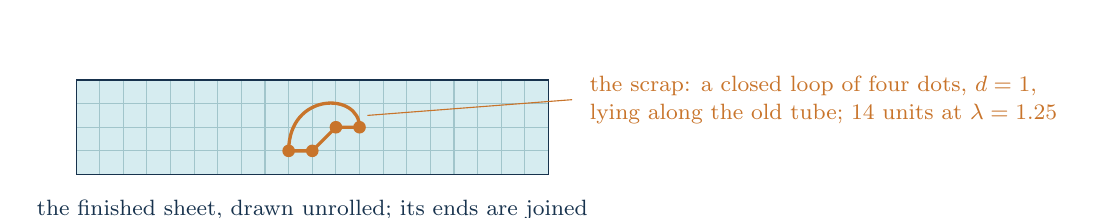
\begin{tikzpicture}[x=1cm,y=1cm,font=\small]
\fill[flatpale] (0,0) rectangle (6.0,1.2);
\draw[flat!45,step=0.3] (0,0) grid (6.0,1.2);
\draw[ink] (0,0) rectangle (6.0,1.2);
\foreach \p in {(2.7,0.3),(3.0,0.3),(3.3,0.6),(3.6,0.6)} {\fill[curl] \p circle (0.08);}
\draw[curl,very thick] (2.7,0.3) -- (3.0,0.3) -- (3.3,0.6) -- (3.6,0.6) .. controls (3.6,1.05) and (2.7,1.05) .. (2.7,0.3);
\draw[curl] (3.7,0.75) -- (6.3,0.95);
\node[font=\footnotesize,text=curl,anchor=west,align=left] at (6.4,0.95) {the scrap: a closed loop of four dots, $d=1$,\\lying along the old tube; 14 units at $\lambda=1.25$};
\node[font=\footnotesize,text=ink] at (3.0,-0.45) {the finished sheet, drawn unrolled; its ends are joined};
\end{tikzpicture}
\caption{The usual leftover. \Exact\ Read from the wiring: a closed loop of four dots with one extra
square and six surplus squares, costing $24\lambda - 16$ (14 at $\lambda=1.25$), its points spanning one
to four of the tube's original columns and lying along the tube. Earlier notes called it a ring
around the tube; the wiring says otherwise. Occasionally a different, 20-unit twist appears instead.}
\end{figure}

\Meas\ Eighty fresh runs in the coldest box, two stores per dot, pre-registered: tubes of 64, 96, 192
and 288 dots. The count of scraps per finished sheet was 0.90, 0.85, 1.05 and 0.95, with a spread of
about 0.2 to 0.4 either way across the twenty runs at each size. A straight line drawn through them is
flat, within that scatter. About one scrap per box, however long the tube.

\begin{figure}[H]
\centering
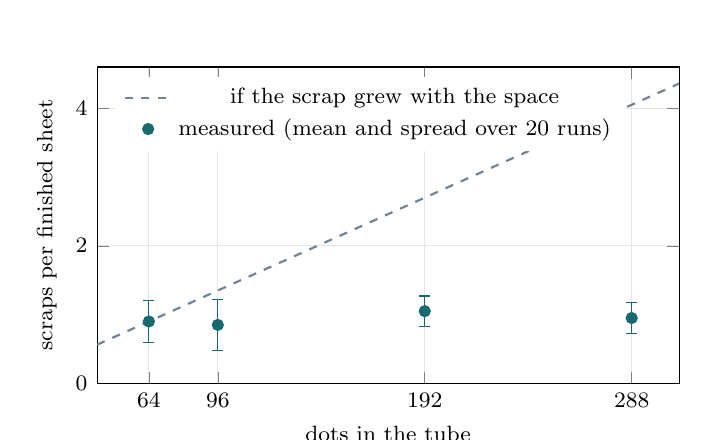
\begin{tikzpicture}
\begin{axis}[width=0.74\linewidth,height=5.6cm,xlabel={dots in the tube},ylabel={scraps per finished sheet},xmin=40,xmax=310,ymin=0,ymax=4.6,xtick={64,96,192,288},grid=both,grid style={gray!20},tick label style={font=\footnotesize},label style={font=\footnotesize},legend style={at={(0.03,0.97)},anchor=north west,font=\footnotesize,draw=none}]
\addplot[ink!60,dashed,thick,domain=40:310] {0.9*x/64};
\addplot[accent,only marks,mark=*,mark options={fill=accent},error bars/.cd,y dir=both,y explicit] coordinates {(64,0.90) +- (0,0.31) (96,0.85) +- (0,0.37) (192,1.05) +- (0,0.22) (288,0.95) +- (0,0.22)};
\legend{if the scrap grew with the space, measured (mean and spread over 20 runs)}
\end{axis}
\end{tikzpicture}
\caption{One scrap, however large. \Meas\ The dashed line is what a leftover growing in step with the
space would look like; the measured counts sit flat. The prediction that it grows, written down
beforehand, failed.}
\end{figure}

\sub{Where does it sit, and why one?}
It is tempting to call the scrap the place where two fronts met and left a seam. \Meas\ That was
pre-registered and tested: the scrap sits neither opposite the start nor at it, and a randomization
check that moves it to every position along the tube finds nothing special about where it landed.
We do not know why the count is about one in this protocol. The technical paper~\cite{tech} says so
under ``not claimed.''

\sub{What the scrap does afterwards}
This paper stops at the count. Three questions follow from it, and they are the subject of the
author's next paper: does a scrap last, or heal away, when the sheet around it is kept warm or is
cooled; does a change that starts in several places at once leave more of them; and if so, is the
leftover a speck or a share. The short version: how many scraps survive depends on how the change
started and how fast the sheet cooled, and more than one prediction written down beforehand failed.

\whyhere{The change leaves a remainder in almost every run, at every size. The pre-registered test
asked the one question that decides what kind of thing it is, and the answer, fixed size, is not the
one the author predicted. It is reported as prominently as the results that went her way.}

\takeaway{The change leaves about one four-dot scrap of the old arrangement per sheet, 14 units,
whatever the size of the tube, sitting anywhere along it. From a single seed the leftover is a
speck. What it does afterwards, and what several seeds leave, is the next paper's question.}

\chapterpage{9 \enspace THE MAP}{Turning the knob}

Everything so far was at one setting of the knob, $\lambda=1.25$, chosen in advance. A single setting
proves little: a result that only holds at one carefully chosen number is the kind of thing the
project's rules forbid. So the whole stretch of the knob was run, from 1.05 to 1.45 in steps of 0.05,
at four sizes, thirty tubes per cell, with the rules fixed first. Then it was run twice more with 120
tubes per cell and fresh random numbers. Each run carries a detector that decides when the change has
happened. It watches the tube for its first 200 sweeps to learn what an unchanged tube looks like, and
only then starts checking, so it cannot record a change earlier than that. The end of this chapter returns to
what this costs.

\begin{figure}[H]
\centering
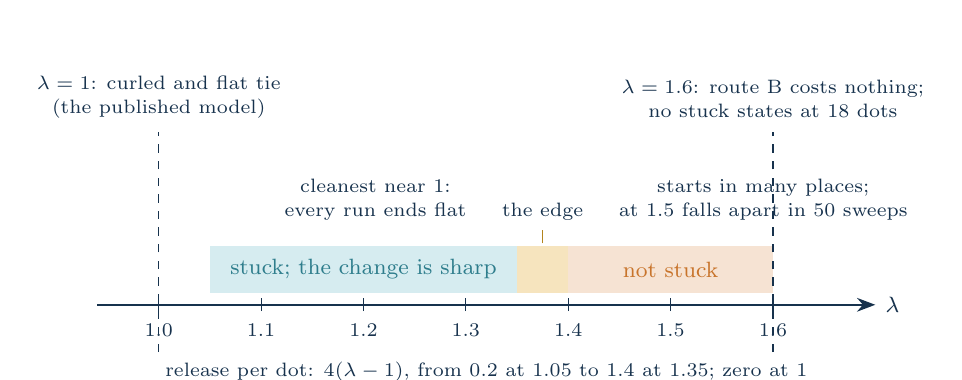
\begin{tikzpicture}[x=13cm,y=1cm,font=\small,>=Stealth]
\draw[->,thick,ink] (0.94,0) -- (1.70,0) node[right,font=\footnotesize] {$\lambda$};
\foreach \x in {1.0,1.1,1.2,1.3,1.4,1.5,1.6} {\draw[ink] (\x,-0.08) -- (\x,0.08); \node[font=\scriptsize,text=ink] at (\x,-0.32) {\x};}
\fill[flatpale] (1.05,0.15) rectangle (1.35,0.75);
\node[font=\footnotesize,text=flat,align=center] at (1.2,0.45) {stuck; the change is sharp};
\fill[sun!30] (1.35,0.15) rectangle (1.40,0.75);
\draw[sun!80!black] (1.375,0.78) -- (1.375,0.95); \node[font=\scriptsize,text=ink,anchor=south] at (1.375,0.95) {the edge};
\fill[curlpale] (1.40,0.15) rectangle (1.60,0.75); \node[font=\footnotesize,text=curl,align=center] at (1.5,0.45) {not stuck};
\draw[dashed,ink] (1.0,-0.6) -- (1.0,2.2); \node[font=\scriptsize,text=ink,align=center,anchor=south] at (1.0,2.25) {$\lambda=1$: curled and flat tie\\(the published model)};
\draw[dashed,ink] (1.6,-0.6) -- (1.6,2.2); \node[font=\scriptsize,text=ink,align=center,anchor=south] at (1.6,2.25) {$\lambda=1.6$: route B costs nothing;\\no stuck states at 18 dots};
\node[font=\scriptsize,text=ink,align=center,anchor=south east] at (1.31,0.95) {cleanest near 1:\\every run ends flat};
\node[font=\scriptsize,text=ink,align=center,anchor=south west] at (1.44,0.95) {starts in many places;\\at 1.5 falls apart in 50 sweeps};
\node[font=\scriptsize,text=ink,align=center] at (1.32,-0.85) {release per dot: $4(\lambda-1)$, from 0.2 at 1.05 to 1.4 at 1.35; zero at 1};
\end{tikzpicture}
\caption{The stretch of the knob that was run. \Meas\ Shaded, where the tube is stuck (more than half
the tubes still at least three-quarters tube after the 200-sweep watch) and the change keeps its
two-signature, dominant-region character. The edge between 1.35 and 1.40 is where the wait drops
below the watch, not where the hill disappears: route B still costs energy until 1.6. \Exact}
\end{figure}

\Meas\ Three things the map shows. First, the tube is stuck at every setting from 1.05 to 1.35 and
at none from 1.40 up, and wherever it is stuck the change keeps the character of Chapter~6: 95 to 100
percent of dots in one signature or the other at the half mark, one connected region holding
most of the flat-like dots. Second, the mean wait follows the counted lottery of Chapter~5 over a
hundred-fold range of waiting times with nothing fitted, drifting above it only where the 200-sweep watch cannot record
shorter waits, and running 15 to 43 percent long near $\lambda = 1$, where the direct move-by-move
count finds no excess. Third, the change is cleanest near the published setting and gets messier as
the knob turns: at 1.05 every one of 120 tubes ended as a perfect flat torus, at 1.25 about 88
percent did, at 1.35 fewer than half, and beyond the edge the change starts in several places at
once in most runs and ends mostly on a sheet with defects.

\begin{figure}[H]
\centering
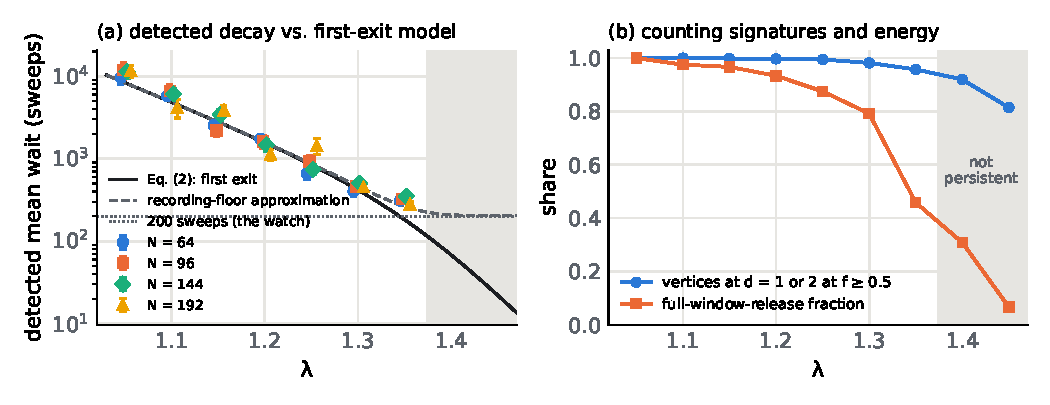
\includegraphics[width=\linewidth]{fig_lambda.pdf}
\caption{The map, measured. (a) Mean detected wait against $\lambda$ at $g=1.5$, four sizes;
the solid line is the counted lottery for the first exit, the dashed line the same prediction as the
200-sweep watch would record it; neither is fitted. Shading marks where the tube is not stuck. (b)
Pooled over sizes: the share of dots in one signature or the other at the half mark, and the share
of runs that released the full amount.}
\end{figure}

\Ours\ There is a trade here. A larger $\lambda$ means a larger
burp per dot but a less patient X and a messier birth; a smaller $\lambda$ means a cleaner change that
releases less. The release is exactly $4(\lambda-1)$ per dot and vanishes at the published setting,
so this family of models has no setting with a large release and a quiet, clean X at once.
\Pub\ At the published setting itself, the model's author has proposed that patches of the network
can sit stuck in a different arrangement~\cite{T24}; the questions asked here could be put to those
patches too.

\sub{Three verdicts, all inconclusive by the letter}
\Meas\ Each of the three maps was scored against rules fixed before it ran, and each failed one of
them: the first on a band for the spread of waits that, with thirty tubes, turned out to be not much
wider than ordinary run-to-run scatter, so a cell could fall outside it by chance alone; the second on an energy check that compared a window average with an exact final
energy and was tripped by the sheet's own thermal jitter; the third on the spread of waits again, in
four cells, two of them on a single tube recorded as waiting 24 and 76 times the predicted mean
(neither of those two was a wait, as the end of this chapter shows). Three runs,
three different criteria tripped, and the physics reading the same each time. The verdict stays
inconclusive, because that is what the rules said, and the measurements stand as the result.

\sub{The long waits that were not waits}
\Meas\ One loose end from these maps looked alarming for a while. The third map recorded two tubes
waiting 24 and 76 times the predicted mean, which a memoryless wait all but forbids. A dedicated
pre-registered test of 10,000 tubes then counted too many long waits and returned the verdict TWO
POPULATIONS. It also found a fast share, 12 to 23 percent of tubes that seemed to change at once, and
190 tubes the detector never caught.

Was something hidden in the model, or was this the detector? It was the detector
(Figure~\ref{fig:watch}). For its first 200 sweeps the detector only watches, to learn how much a
resting tube jiggles, and then it sets its bar at three times that jiggle. A tube that changes
\emph{during} the watch teaches it that large swings are normal.

\begin{figure}[H]
\centering
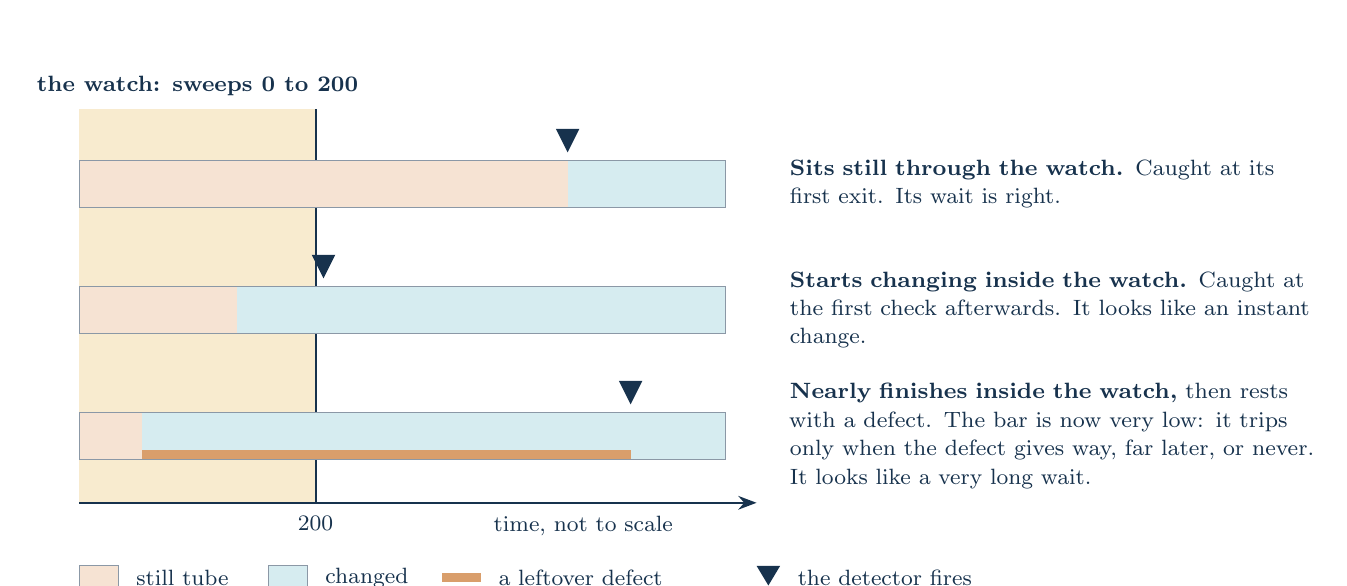
\begin{tikzpicture}[x=1cm,y=1cm,font=\footnotesize,>=Stealth]
% the watch
\fill[sun!22] (0,-0.25) rectangle (3.0,4.75);
\node[text=ink,font=\footnotesize\bfseries] at (1.5,5.05) {the watch: sweeps 0 to 200};
\draw[ink,thick] (3.0,-0.25) -- (3.0,4.75);
\draw[->,thick,ink] (0,-0.25) -- (8.6,-0.25);
\node[text=ink,anchor=north] at (3.0,-0.3) {200};
\node[text=ink,anchor=north] at (6.4,-0.3) {time, not to scale};
% row A: waits past the watch
\fill[curlpale] (0,3.5) rectangle (6.2,4.1); \fill[flatpale] (6.2,3.5) rectangle (8.2,4.1); \draw[ink!50] (0,3.5) rectangle (8.2,4.1);
\fill[ink] (6.2,4.2) -- (6.05,4.5) -- (6.35,4.5) -- cycle;
\node[text=ink,align=left,anchor=west,text width=6.6cm] at (8.9,3.8) {\textbf{Sits still through the watch.} Caught at its first exit. Its wait is right.};
% row B: begins to change inside the watch
\fill[curlpale] (0,1.9) rectangle (2.0,2.5); \fill[flatpale] (2.0,1.9) rectangle (8.2,2.5); \draw[ink!50] (0,1.9) rectangle (8.2,2.5);
\fill[ink] (3.1,2.6) -- (2.95,2.9) -- (3.25,2.9) -- cycle;
\node[text=ink,align=left,anchor=west,text width=6.6cm] at (8.9,2.2) {\textbf{Starts changing inside the watch.} Caught at the first check afterwards. It looks like an instant change.};
% row C: nearly finishes inside the watch
\fill[curlpale] (0,0.3) rectangle (0.8,0.9); \fill[flatpale] (0.8,0.3) rectangle (8.2,0.9); \fill[curl!70] (0.8,0.3) rectangle (7.0,0.42); \draw[ink!50] (0,0.3) rectangle (8.2,0.9);
\fill[ink] (7.0,1.0) -- (6.85,1.3) -- (7.15,1.3) -- cycle;
\node[text=ink,align=left,anchor=west,text width=6.6cm] at (8.9,0.6) {\textbf{Nearly finishes inside the watch,} then rests with a defect. The bar is now very low: it trips only when the defect gives way, far later, or never. It looks like a very long wait.};
% key
\fill[curlpale] (0,-1.35) rectangle (0.5,-1.05); \draw[ink!50] (0,-1.35) rectangle (0.5,-1.05); \node[text=ink,anchor=west] at (0.6,-1.2) {still tube};
\fill[flatpale] (2.4,-1.35) rectangle (2.9,-1.05); \draw[ink!50] (2.4,-1.35) rectangle (2.9,-1.05); \node[text=ink,anchor=west] at (3.0,-1.2) {changed};
\fill[curl!70] (4.6,-1.26) rectangle (5.1,-1.14); \node[text=ink,anchor=west] at (5.2,-1.2) {a leftover defect};
\fill[ink] (8.75,-1.3) -- (8.6,-1.05) -- (8.9,-1.05) -- cycle; \node[text=ink,anchor=west] at (9.0,-1.2) {the detector fires};
\end{tikzpicture}
\caption{Three tubes, one detector. \Exact\ The detector's rule is the same for all three; what differs
is what each tube did while the detector was still watching.}
\label{fig:watch}
\end{figure}

\MeasX\ Every run saved two readings that do not depend on the detector's bar: how far the tube had
converted when the watch ended, and when a quarter of it had converted. Read afterwards from those
saved rows (a reading made after the fact, not a pre-registered test), the puzzle comes apart. The 190
tubes never caught had all finished at least three-quarters of the change inside the watch. The two
extreme waits were tubes already 75 and 88 percent converted when the watch ended, resting on a sheet
with defects. The fast share is tubes whose first exit came inside the watch, about as many as the
counted lottery says there should be. And the test's yardstick for a typical wait, taken with the fast
share included, came out too short, which pushed ordinary long waits past its cutoff.

The verdict stands as scored; what it reported on was its own detector. Three long waits in one group
of 4,000, at $\lambda = 1.30$ and 64 dots, were not explained this way, so we replayed that whole group
move for move from its saved starting numbers, this time recording everything, with the rules for
reading it written down first. \Meas\ One of the three was the detector again. The other two
looked like perfect tubes every time the replay looked, which was once every five sweeps. So we
replayed them once more and looked after every single sweep. \MeasX\ One had sat, perfect, for
about twelve times the average wait. The other had slipped out for three sweeps between two looks
and come back, about seven average waits in, so its long wait was the spacing of the looks. At no
sweep did any tube hold more squares than a perfect tube, which a second curl would need.
\Meas\ Neither written guess about the three held (a hidden second curl; the detector three times
over). Timed with no detector at all, the 4,000 first exits follow the counted lottery to within 7
percent, and one comes later than ten average waits, which chance allows about one time in six.

\whyhere{The project's first success condition is no cherry-picking: a family of rules may be
explored, but only along knobs fixed in advance, and every setting run is published. The map is that
rule applied, and it also locates where the stand-in for X stops being stable for now.}

\takeaway{From $\lambda=1.05$ to 1.35 the tube waits and then opens sharply; at 1.40 it no longer
waits. The change is cleanest nearest the published setting and leaves more defects as the knob
turns. Three pre-registered maps each came back inconclusive on a different rule while reading the
same physics, and the long waits that seemed to point to something hidden were the detector, or
simply long.}

\chapterpage{10 \enspace THE EDGES}{Where the simulations stop, and what lies past each edge}

Every knob the toy has was turned only so far. This chapter is the honest map of the box: for each
knob, what was run, why it stopped there, and what is on the other side, with the kind of knowledge
marked. ``Unknown'' means no one has looked.

\begin{figure}[H]
\centering
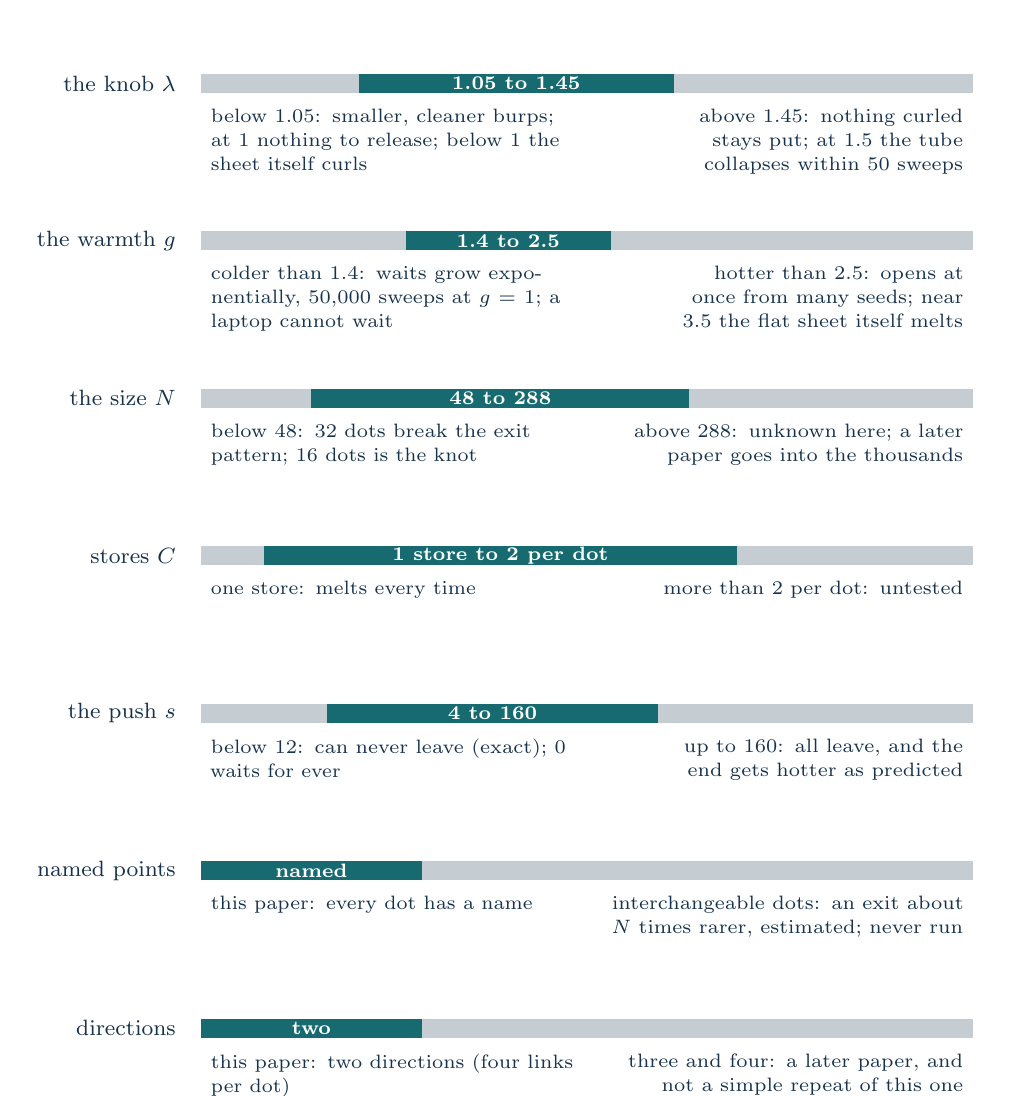
\begin{tikzpicture}[x=1cm,y=1cm,font=\footnotesize]
% rows: label at x=0, bar from 2.6 to 12.4
\foreach \yy/\name/\lo/\hi/\ltext/\rtext/\inside in {
 0/the knob $\lambda$/4.6/8.6/{below 1.05: smaller, cleaner burps; at 1 nothing to release; below 1 the sheet itself curls}/{above 1.45: nothing curled stays put; at 1.5 the tube collapses within 50 sweeps}/{1.05 to 1.45},
 -2.0/the warmth $g$/5.2/7.8/{colder than 1.4: waits grow exponentially, 50,000 sweeps at $g=1$; a laptop cannot wait}/{hotter than 2.5: opens at once from many seeds; near 3.5 the flat sheet itself melts}/{1.4 to 2.5},
 -4.0/the size $N$/4.0/8.8/{below 48: 32 dots break the exit pattern; 16 dots is the knot}/{above 288: unknown here; a later paper goes into the thousands}/{48 to 288},
 -6.0/stores $C$/3.4/9.4/{one store: melts every time}/{more than 2 per dot: untested}/{1 store to 2 per dot},
 -8.0/the push $s$/4.2/8.4/{below 12: can never leave (exact); 0 waits for ever}/{up to 160: all leave, and the end gets hotter as predicted}/{4 to 160},
 -10.0/named points/2.6/5.4/{this paper: every dot has a name}/{interchangeable dots: an exit about $N$ times rarer, estimated; never run}/{named},
 -12.0/directions/2.6/5.4/{this paper: two directions (four links per dot)}/{three and four: a later paper, and not a simple repeat of this one}/{two}} {
 \node[anchor=east,text=ink] at (2.4,\yy) {\name};
 \draw[ink!25,line width=7pt] (2.6,\yy) -- (12.4,\yy);
 \draw[accent,line width=7pt] (\lo,\yy) -- (\hi,\yy);
 \node[text=white,font=\scriptsize\bfseries] at ({(\lo+\hi)/2},\yy) {\inside};
 \node[anchor=north west,text=ink,font=\scriptsize,text width=4.6cm,align=left] at (2.6,\yy-0.2) {\ltext};
 \node[anchor=north east,text=ink,font=\scriptsize,text width=4.6cm,align=right] at (12.4,\yy-0.2) {\rtext};
}
\end{tikzpicture}
\caption{The box, knob by knob. Each teal bar is the stretch of a knob where tubes were actually
simulated for this paper; the gray is the knob's range as far as anything is known about it; the notes
say what lies past each edge. You can turn the first five knobs yourself in the interactive companion
to this figure, \href{https://claude.ai/artifact/F4sBf955J5ZT7rCq8uebW8}{The Tube's Curling Ladder}:
its exact numbers follow you to any setting, and its measured results appear only inside the teal
bars. Details and the kind of knowledge behind each note follow.}
\label{fig:box}
\end{figure}

\sub{The knob $\lambda$: 1.05 to 1.45}
Below 1.05 the burp gets smaller and cleaner, not longer-awaited. \Exact\ The wait saturates as the
knob approaches 1 (the counted lottery gives about 8,300 sweeps at 1.05 and about 14,000 at 1.001),
while the release shrinks to nothing at exactly 1, where curled and flat tie and the tube is no
longer above anything. Below 1 the ladder flips. \MeasX\ In a rehearsal the author calls the backwards
reaction, a perfect flat sheet at $\lambda<1$ sat at zero for hundreds to thousands of sweeps and then
curled, one direction first, releasing energy in steps that landed on the exact rungs of the ladder.
Above 1.45, \Meas\ at 1.5 the tube falls apart within 50 sweeps in every run; \Exact\ at 1.6 route B
costs nothing and at 18 dots no stuck state above flat exists; by a knob setting of 5 to 10 the model
behaves as one with a third square simply forbidden. Nothing curled is stable for now out there.

\sub{The warmth $g$: 1.4 to 2.5, with the maps at 1.5}
\Exact\ Colder, the wait grows like $e^{12/g}$: about 50,000 sweeps at $g=1$ and nearly three million at
$g = 0.75$. \MeasX\ At $g=1$, two of four tubes were still tubes after 30,000 sweeps. A laptop cannot
wait long enough below about 1, which is why the knob stopped there. Hotter, the tube opens almost at
once and from many places, and near $g \approx 3.5$ the flat sheet itself melts into the random phase;
that melting point is the one the reservoir estimate of Chapter~7 used. How that melting point
moves with the size of the sheet is taken up in a later paper; until then every warm result carries a
size caveat.

\sub{The size $N$: 48 to 288 dots}
The upper limit was run time on one laptop and the choice to spend compute on repeats rather than
size. \Exact\ The exit count was certified at 48 through 288; the control at 32 dots breaks the
pattern, and 16 dots is the knot. \Meas\ The front's speed fell roughly as the size to the power
$-0.7$, so longer tubes take longer to finish. \Ours\ Whether the wait itself grows, stays flat or
falls with size depends on the clock the model does not fix (Chapter~5). The technical paper claims
nothing beyond 288. Networks into the thousands of dots are the subject of a later paper on the
scrap.

\sub{Stores $C$: one to two per dot}
\Meas\ A single store melts every tube; two per dot leaves clean sheets with one scrap. Colder boxes
than two per dot were not tried. The store balances were not saved, so they cannot be turned into a
calibrated temperature after the fact.

\sub{The push $s$: 4 to 16, then 12 to 160}
\Exact\ Below 12 nothing can leave by single swaps, at the certified sizes; a tube with nothing to
spare waits for ever, which is now a permanent test in the code. \MeasX\ Above, pushes of 12 to 160
units at 64 dots all left, and the hotter the box the more disordered the sheet it ended with, with
the ending predicted from the model's equilibrium curve before the run: 0.97 squares per dot measured
against 0.95 predicted at the smallest push, 0.81 against 0.81 at the largest. Give it far more and it
melts.

\sub{Named or interchangeable dots}
\Ours\ Every run treats dot 17 as a different thing from dot 41. If instead two networks that differ
only by renaming count as one, as identical particles do, every energy stays the same and so does the
12, but each exit from the perfect tube would be accepted about $N$ times less often, because the
tube has many symmetries and the state one swap away has two. The waiting time would then grow with
size instead of staying flat. The knob exists, was decided on, and was not turned for this paper.

\sub{Directions: two}
Four links per dot give two directions. Six and eight links give three and four
(Figure~\ref{fig:directions}), closer to the three directions of space, and they are the subject of a
later paper. The tease: a curled direction in three dimensions does not open the way the tube does,
and the reason is partly exact and partly still open.

\sub{The route}
The published route starts from a random tangle; this paper starts from an ordered tube. \Meas\ Both
were run. From randomness at $\lambda \geq 1$: one hump, no sign of a release at these sizes. From the tube at
$\lambda>1$: a hill, a push, a burp. The two routes are different questions, and the toy gives them
different answers.

\takeaway{The box is small and its edges are known. Past most of them lies either an exact statement
(nothing below 12 can leave; nothing is below flat), a later measurement with its own paper, or a
plain ``unknown.'' The one edge the toy cannot push on its own is the clock.}

\chapterpage{11 \enspace WHAT WE HAVE LEARNED, AND WHAT COMES NEXT}{A mechanism we can price, and two questions it opens}

Return one last time to the 96-dot tube. Its excess energy is exact: 96 units. The cheapest way out is
exact: 12 units, the same at every size certified. The counted lottery predicts when it first leaves,
and the tube keeps that appointment over a ninety-fold range of waits. Halfway through, 99 dots in
100 belong to one arrangement or the other. When it finishes flat, it gives off exactly one unit per
dot, and sealed, the energy is followed to the unit into stores and into a four-dot scrap. The whole
chain holds at every setting of the knob from 1.05 to 1.35.

\sub{What the toy shows about this kind of change}
\Ours\ What the toy shows is that a graph energy one coefficient away from a published model of
emergent geometry contains a change with the shape of the idea in Chapter~1: a specific curled arrangement, stable
for now, that opens sharply from a seed with a fixed push, releases a definite and growing burp, and
leaves a fixed remainder. It shows that this change does not exist at the curvature setting and
needs the knob above 1. It shows that the release has to have somewhere to go or it undoes the
change. And it shows that the remainder, from one seed, is a speck.

What it does not show is anything about reality. A toy can show that a mechanism is possible or
impossible within a class of models; that is the whole claim. \Claim\ The author claims that reality
works this way, and people can argue. The model's part is to make the claim concrete enough to be
wrong in specific ways, and several of those ways have now been tried: the remainder did not grow,
the single-front law was not established, three maps were inconclusive by their own rules, and a
test that reported a second population of waits turned out to be reporting on its own detector.

\sub{What another researcher can build on}
Some parts are exact or complete finite listings: the ladder, the 12, the three reachable
arrangements, the topology of 120 endpoints. Their scope is the stated rules, sizes and the
correctness of the code, which is tested against independent calculations. Other parts are
measurements with variation between repeated runs, where a hundred dots in one run are not a hundred
experiments. Tests written down before the data are marked pre-registered; the Arrhenius scan, the
push threshold and the endpoint-energy reading are exploratory and say so. Interpretations are the
author's and her assistants' and have not been checked by a physicist.

Even what to count is a choice. The simulations count named dots. Counting each wiring once, with the
names removed, leaves every energy alone and changes the rates, most for the symmetric arrangements
that are easiest to calculate with and that nothing is ever in. That knob is decided and not yet
turned.

\sub{What the next round of this experiment should record}
Time every tube from its first sweep, with no watch, and save every exit and return. Measure both ways
around the finished torus as the size grows. Record each store's balance, so that the bath's
temperature can be read and not estimated. Hold out the largest size and predict it from the smaller
ones before it runs.

\sub{What comes next}
The question that began the work survives its first test. Can an organized arrangement give way
sharply, release energy and leave a remainder? In this small laboratory it can, and the first step
can be priced to the unit. Two things were left standing at the edge of what this paper measured, and
each has a paper of its own coming, with its predictions written down first.

\textbf{The scrap.} A scrap is the only thing in the new space that still carries the old
arrangement, so the next paper, \emph{What the burp leaves behind}, asks what it takes to keep one.
\Meas\ One result: the scrap counted here is not permanent. Cool the new sheet slowly enough and it
heals away, while another kind of leftover survives every cooling we could run.

\textbf{Three directions.} The tube has one open direction, and space has three, so the paper after
that, \emph{How curled directions open}, runs the same rules with six links per dot. \Meas\ One
result: the tube's trick does not carry over. Here one fixed push set off the whole change. There each
curled direction sits behind its own wall, and one push has never opened them all.

\begin{center}
{\color{ink}\Large\bfseries A push of twelve units opens a tube. What opens a space?}
\end{center}

\par\Needspace{14\baselineskip}\vspace{1.4em}
{\color{ink}\LARGE\bfseries Continuing into the technical paper}\par
\vspace{0.6em}

This edition follows the technical paper~\cite{tech}, which holds the equations, tables, uncertainty
calculations and full references. Every number above is taken from it or from the project's record,
and the kinds-of-statement tags follow the project's own rule that no statement is promoted from one
kind to another without a dated note saying why. Its sections run in the same order as the chapters here:
the model and its exact results (Chapters~2 and~3), the cost of leaving (4), the first exit (5), the
conversion (6), the sealed system (7 and~8) and the dependence on $\lambda$ (9).

\sub{A few translations for the next step}
\renewcommand{\arraystretch}{1.3}
\begin{tabularx}{\linewidth}{@{}>{\bfseries}p{0.24\linewidth}X@{}}
\toprule
In the paper & What to keep in mind\\
\midrule
$N$ & Number of dots. The running example uses $N=96$.\\
Torus & Any grid that wraps both ways. The flat torus is the sheet, the curled torus is the tube, and the smallest one, curled both ways, is the knot.\\
$4\times L$ & Four steps around the short wrap and $L$ around the other, $L$ even and above 4. $4\times4$ is the knot.\\
$\lambda$ and $g$ & Lambda sets the price of a surplus square and so the whole ladder; $g$ is the bath's warmth, which sets how often an uphill swap is accepted.\\
$H = 16(N-S) + 4\lambda X$ & The price list: $S$ squares, $X$ surplus squares. Zero on the flat sheet; $4(\lambda-1)$ per dot on the tube.\\
$\Delta E^\ddagger = 32 - 16\lambda$ & The rim: the cost of route A, 12 at $\lambda=1.25$. Route B costs $64 - 40\lambda$.\\
$d$ & The direction count: pairs of links at a dot that close no square. Sheet 2, tube 1, knot 0. A counting signature, not a certified geometry.\\
$f$ & The progress meter, 0 for the tube and 1 for the sheet. Disorder raises it too.\\
Arrhenius law & Uphill events becoming much rarer as the bath cools, as $e^{-\text{cost}/g}$. Here its two ingredients are counted, not fitted.\\
Memoryless & The chance of leaving is the same on every attempt, like rolling a die until a six comes up; a long wait so far makes leaving no nearer.\\
Metastable & Stable for now: every single move out costs energy. The map's edge near 1.37 is where the wait drops below the watch, not where that stops being true.\\
Microcanonical & Sealed: energy conserved, the temperature read off the stores rather than imposed.\\
Pre-registered & The prediction and the rules of the test were committed before the run. Exploratory runs say so.\\
95\% interval & A range from a statistical procedure that, under its assumptions, covers the truth 95 times in 100.\\
\bottomrule
\end{tabularx}

\sub{Where the evidence is recorded}
The technical manuscript and its methods supplement are in
\href{https://github.com/EmilySmithCreate/RecreationalPhysics/tree/main/docs/papers/curled_torus}{the recorded repository version},
and the \href{https://github.com/EmilySmithCreate/RecreationalPhysics/blob/main/docs/papers/curled_torus/supplement.md}{supplement}
maps every claim to code, configurations and result files. Experiment labels in that record: T7 and
T8 (the decay and the map), T9 (the sealed reservoir), T10 and T11 (the scrap and its position), T22
(exits counted move by move), T38 (the long-wait test). The questions teased above, what the scrap
does afterwards, larger networks and more directions, have their own labels in the record and their
own papers. The push threshold covers 48 to 192 dots and the exit enumeration 48 to 288; neither
extends to other sizes.

\sub{Disclosure}
The author used Claude (Anthropic) and ChatGPT/Codex (OpenAI) to assist with code, analysis and
writing, and is responsible for the result. This edition was drafted with Claude from the corrected
manuscript and the project's record. Its analogies and pictures introduce no new experiments or
evidence. No physicist has reviewed any of it.

\renewcommand{\refname}{Sources}
\begin{thebibliography}{99}\small
% Sources 1 to 8 are the technical paper's reference list in its order, so that a number means the same
% source in both documents; 9 to 12 are this edition's own.
\bibitem{T17} C.~A. Trugenberger, \emph{Combinatorial quantum gravity: geometry from random bits}, 
J.\ High Energy Phys.\ \textbf{09} (2017) 045, arXiv:1610.05934. Cited as in the technical paper.
\bibitem{KTB19} C.~Kelly, C.~A. Trugenberger, and F.~Biancalana, \emph{Self-assembly of geometric space
from random graphs}, Class.\ Quantum Grav.\ \textbf{36}, 125012 (2019), arXiv:1901.09870.
\bibitem{T25} C.~A. Trugenberger, \emph{Networks as the fundamental constituents of the universe},
J.\ Phys.\ Complex.\ \textbf{6}, 042001 (2025), arXiv:2512.17676.
\bibitem{GV21} A.~Gorsky and O.~Valba, \emph{Interacting thermofield doubles and critical behavior in
random regular graphs}, Phys.\ Rev.\ D \textbf{103}, 106013 (2021), arXiv:2101.04072.
\bibitem{Kelly22} C.~Kelly, \emph{Emergent geometry and discrete curvature in random graphs}, Ph.D.
thesis, Heriot-Watt University (2022), \url{https://www.ros.hw.ac.uk/handle/10399/4591}.
\bibitem{T24} C.~A. Trugenberger, \emph{Dark matter and dark energy in combinatorial quantum gravity},
arXiv:2409.09385 (2024).
\bibitem{Creutz83} M.~Creutz, \emph{Microcanonical Monte Carlo simulation}, Phys.\ Rev.\ Lett.\ \textbf{50},
1411 (1983). Cited as in the technical paper; we have not read it in full.
\bibitem{C77} S.~Coleman, \emph{Fate of the false vacuum: semiclassical theory}, Phys.\ Rev.\ D
\textbf{15}, 2929 (1977). Described here from general knowledge of the paper; we have not read it in
full.
\bibitem{tech} E.~Smith, \emph{The curled torus burps: activated escape and conversion in a graph model
of emergent geometry}, technical manuscript, 10 October 2026,
\href{https://github.com/EmilySmithCreate/RecreationalPhysics/tree/main/docs/papers/curled_torus}{in the project repository}.
\bibitem{Planck18} Planck Collaboration, \emph{Planck 2018 results. VI. Cosmological parameters},
Astron.\ Astrophys.\ \textbf{641}, A6 (2020), arXiv:1807.06209.
\bibitem{search} The written search behind this sentence, 10 October 2026: where we looked, with what
terms, and what came closest. File
\texttt{docs/reading/notes/2026-10-10\_prior\_work\_lambda\_above\_one.md} in
\href{https://github.com/EmilySmithCreate/RecreationalPhysics}{the project repository}.
\bibitem{KT19} C.~Kelly and C.~A. Trugenberger, \emph{Combinatorial quantum gravity: emergence of
geometric space from random graphs}, arXiv:1811.12905 (2018).
\end{thebibliography}

\noindent{\small Sources 1 to 8 carry the same numbers as in the technical paper~\cite{tech}; 9 to 12 are this
edition's own.}

\end{document}
